% Preámbulo
\documentclass[letterpaper]{article}
\usepackage[utf8]{inputenc}
\usepackage[spanish]{babel}

\usepackage{enumitem}
\usepackage{titling}

% Símbolos
	\usepackage{amsmath}
	\usepackage{amssymb}
	\usepackage{amsthm}
	\usepackage{amsfonts}
	\usepackage{mathtools}
	\usepackage{bbm}
	\usepackage[thinc]{esdiff}
	\allowdisplaybreaks

% Márgenes
	\usepackage
	[
		margin = 1in
	]
	{geometry}

% Imágenes
	\usepackage{float}
	\usepackage{graphicx}
	\graphicspath{{imagenes/}}
	\usepackage{subcaption}

% Ambientes
	\usepackage{amsthm}

	\theoremstyle{definition}
	\newtheorem{ejercicio}{Ejercicio}

	\newtheoremstyle{lemathm}{4pt}{0pt}{\itshape}{0pt}{\bfseries}{ --}{ }{\thmname{#1}\thmnumber{ #2}\thmnote{ (#3)}}
	\theoremstyle{lemathm}
	\newtheorem{lema}{Lema}

	\newtheoremstyle{lemathm}{4pt}{0pt}{\itshape}{0pt}{\bfseries}{ --}{ }{\thmname{#1}\thmnumber{ #2}\thmnote{ (#3)}}
	\theoremstyle{lemathm}
	\newtheorem{sol}{Solución}
	
	\newtheoremstyle{lemathm}{4pt}{0pt}{\itshape}{0pt}{\bfseries}{ --}{ }{\thmname{#1}\thmnumber{ #2}\thmnote{ (#3)}}
	\theoremstyle{lemathm}
	\newtheorem{theo}{Teorema}

	\newtheoremstyle{lemademthm}{0pt}{10pt}{\itshape}{ }{\mdseries}{ --}{ }{\thmname{#1}\thmnumber{ #2}\thmnote{ (#3)}}
	\theoremstyle{lemademthm}
	\newtheorem*{lemadem}{Demostración}

% Macros
	\newcommand{\sumi}[2]{\sum_{i=#1}^{#2}}
	\newcommand{\dint}[2]{\displaystyle\int_{#1}^{#2}}
	\newcommand{\inte}[2]{\int_{#1}^{#2}}
	\newcommand{\dlim}{\displaystyle\lim}
	\newcommand{\limtoinf}[1]{\lim_{#1\to\infty}}
	\newcommand{\dlimtoinf}[1]{\displaystyle\lim_{#1\to\infty}}
	\newcommand{\limtozero}[1]{\lim_{#1\to0}}
	\newcommand{\limh}{\lim_{h\to0}}
	\newcommand{\ddx}{\dfrac{d}{dx}}
	\newcommand{\txty}{\text{ y }}
	\newcommand{\txto}{\text{ o }}
	\newcommand{\Txty}{\quad\text{y}\quad}
	\newcommand{\Txto}{\quad\text{o}\quad}
	\newcommand{\si}{\text{si}\quad}

	\newcommand{\etiqueta}{\stepcounter{equation}\tag{\theequation}}
	\newcommand{\tq}{:}
	\renewcommand{\o}{\circ}
	\newcommand*{\QES}{\hfill\ensuremath{\blacksquare}}
	\newcommand*{\qes}{\hfill\ensuremath{\square}}
	\newcommand*{\QESHERE}{\tag*{$\blacksquare$}}
	\newcommand*{\qeshere}{\tag*{$\square$}}
	\newcommand*{\QED}{\hfill\ensuremath{\blacksquare}}
	\newcommand*{\QEDHERE}{\tag*{$\blacksquare$}}
	\newcommand*{\qel}{\hfill\ensuremath{\boxdot}}
	\newcommand*{\qelhere}{\tag*{$\boxdot$}}
	\renewcommand*{\qedhere}{\tag*{$\square$}}

	\newcommand{\suc}[1]{\left(#1_n\right)_{n\in\N}}
	\newcommand{\en}[2]{\binom{#1}{#2}}
	\newcommand{\upsum}[2]{U(#1,#2)}
	\newcommand{\lowsum}[2]{L(#1,#2)}
	\newcommand{\abs}[1]{\left| #1 \right| }
	\newcommand{\bars}[1]{\left \| #1 \right \| }
	\newcommand{\pars}[1]{\left( #1 \right) }
	\newcommand{\bracs}[1]{\left[ #1 \right] }
	\newcommand{\inprod}[1]{\left\langle #1 \right\rangle }
    \newcommand{\norm}[1]{\left\lVert#1\right\rVert}
	\newcommand{\floor}[1]{\left \lfloor #1 \right\rfloor }
	\newcommand{\ceil}[1]{\left \lceil #1 \right\rceil }
	\newcommand{\angles}[1]{\left \langle #1 \right\rangle }
	\newcommand{\set}[1]{\left \{ #1 \right\} }
	\newcommand{\norma}[2]{\left\| #1 \right\|_{#2} }

	\newcommand{\NN}{\mathbb{N}}
	\newcommand{\QQ}{\mathbb{Q}}
	\newcommand{\RR}{\mathbb{R}}
	\newcommand{\ZZ}{\mathbb{Z}}
	\newcommand{\PP}{\mathbb{P}}
    \newcommand{\EE}{\mathbb{E}}
	\newcommand{\1}{\mathbbm{1}}
	\newcommand{\eps}{\varepsilon}
	\newcommand{\ttF}{\mathtt{F}}
	\newcommand{\bfF}{\mathbf{F}}

	\newcommand{\To}{\longrightarrow}
	\newcommand{\mTo}{\longmapsto}
	\newcommand{\ssi}{\Longleftrightarrow}
	\newcommand{\sii}{\Leftrightarrow}
	\newcommand{\then}{\Rightarrow}

	\newcommand{\pTFC}{{\itshape 1er TFC\/}}
	\newcommand{\sTFC}{{\itshape 2do TFC\/}}


% Datos
    \title{Cálculo III \\ Tarea I}
    \author{Rubén Pérez Palacios Lic. Computación Matemática\\Profesor: Dr. Luis Hernández Lamoneda }
    \date{\today}

% DOCUMENTO
\begin{document}
	\maketitle

	\begin{enumerate}
		\item Prueba que si $X$ y $Y$ son ortogonales en $\RR^n$ entonces
		
		\[\norm{X+Y}^2 = \norm{X}^2 + \norm{Y}^2.\]

		\begin{proof}
			Sean $X,Y\in \RR^n$ ortogonales. Por la relación del producto interior y la norma euclideana tenemos que

			\[\norm{X+Y}^2 = \inprod{X+Y,X+Y},\]

			por linealidad del producto punto eso es

			\[\norm{X+Y}^2 = \inprod{X,X} + \inprod{X,Y} + \inprod{Y,Y},\]

			de nuevo por lo relación del producto interior y la norma euclideana obtenemos

			\[\norm{X+Y}^2 = \norm{X}^2 + 2\inprod{X,Y} + \norm{Y}^2,\]

			finalmente al ser $X$ y $Y$ ortogonales esto es si y sólo $\inprod{X,Y}=0$, por lo tanto concluimos que

			\[\norm{X+Y}^2 = \norm{X}^2 + \norm{Y}^2.\]
		\end{proof}
		\item Imagina un cubo $n-$dimensional en $\RR^n$ con tamaño de lado $c:0$, el cuál consiste de todos los puntos $X = \pars{x_1,x_2,\cdots,x_n}$ con
		
		\[0\leq x_k\leq c, \quad k=1,\cdots,n.\]

		\begin{enumerate}
			\item Encuentra el punto $P$ en el cubo tal que su norma es la más grande. Llama a este punto la esquina más alejada del cubo.
			\begin{sol}
				Sea $X = \pars{x_1,x_2,\cdots,x_n}$ un punto en el cubo, veamos que

				\[\norm{X} = \norm{\sum_{i=1}^n x_ie_i},\]

				donde $e$ es la base canonica. Ahora por subatividad tenemos que

				\[\norm{X} \leq \sum_{i=1}^n \norm{x_ie_i},\]

				por definición de $e_i$ y la norma euclideana esto es

				\[\norm{X} \leq \sum_{i=1}^n x_i, \text{ al ser positivos los $x_i$'s omtimos el módulo}.\]

				Ahora por definición $x_i \leq c$ para todo $i$, por lo tanto

				\[\norm{X} \leq \sum_{i=1}^n c,\]

				por definición de $e_i$ y la norma euclideana esto es

				\[\norm{X} \leq \sum_{i=1}^n \norm{c\pars{e_i}},\]

				finalmente al tener la base canónica vectores unitarios obtenemos

				\[\norm{X} \leq c\sqrt{n}.\]

				Ahora el punto $C = (c,c,\cdots,c)$ en el cubo tiene como norma

				\[\norm{C} = c\sqrt{n}.\]

				Con lo que obtenemos que $C$ es un punto en el cubo cuya norma es la más grande. 
				
				Supongamos que existe otro punto $D = \pars{d_1,\cdots, d_n}$ en el cubo y distinto a $C$ cuya norma sea igual a la de $C$, por definición del cubo algún $d_j$ deberá ser menor a $c$. Luego que al ser $0\leq d_i\leq c$ entonces $d_i^2 \leq c^2$ y además como $d_j^2 < c^2$ entonces

				\[\sum_{i=1}^n d_i^2 < \sum_{i=1}^n c^2,\]

				finalmente como la raiz cuadrado es una función monótona y creciente concluimos que

				\[\norm{D} < \norm{C},\]

				lo cuál es una contradicción. Con lo que concluimos que $C$ es el punto más alejado.
			\end{sol}
			\item ¿Cuál es el valor de $c$ tal que la esquina más alejada del cubo está en la esfera unitaria $(\norm{X}=1)$?
			
			\begin{sol}
				Por definición de $C$ tenemos que

				\[\norm{C} = c\sqrt{n},\]

				luego $C$ está en la esfera unitaria ssi $\norm{C} = 1$ por lo tanto $c$ es tal que

				\[c\sqrt{n} = 1,\]

				por lo tanto

				\[c = \frac{1}{\sqrt{n}}.\]

			\end{sol}
			\item Fijando la esquina más alejada del cubo en la esfera unitaria, ¿qué le pasá al tamaño $c$ del lado mientras que la dimensión $n$ tiende a infinito?
			
			\begin{sol}
				Cómo

				\[\limtoinf{n} \frac{1}{\sqrt{n}} = 0,\]

				entonces si $C$ está en la bola unitaria obtenemos que

				\[\limtoinf{n} c = 0.\]
			\end{sol}
		\end{enumerate}
		\item Sea $W_1 = \pars{1,1,1,0}$ y $W_2 = \pars{0,1,1,1}$. Encuentra dos vectores independientes y ortogonales a $W_1$ y $W_2$.
		
		\begin{sol}
			Sea $V\in \RR^N$ un vector ortogonal a $W_1$ y a $W_2$ entonces por definición

			$\inprod{V,W_1} = \inprod{V,W_2} = 0$.

			Lo cuál nos induce el siguiente sistema de ecuaciones

			\begin{align*}
				V_1 + V_2 + V_3 &= 0,\\
				V_2 + V_3 + V_4 &= 0.
			\end{align*}

			Del sistema de ecuaciones anterior obtenemos

			\[V_1 - V_4 = 0,\]

			es decir

			\[V_1 = V_4.\]

			Luego si $V_1 = 0$ y $V_2 = 1$ obtenemos $V=\pars{0,1,-1,0}$. En cambio si $V_1 = 1$ y $V_2 = -1$ entonces $V = \pars{1,-1,0,1}$. Por construcción ambos vectores son ortogonales a $W_1$ y a $W_2$, pero además al tener ambos vectores en una entrada igual a $0$ y el otro no culimna en que son independientes.
		\end{sol}

		\item En nuestra prueba de la desigualdad de Cauchy-Schwarz, en el teorema $1.12$ usamos que si $U$ es un vector unitario, entonces
		
		\[0\leq \norm{V-\inprod{U,V}U}^2 = \norm{V}^2 - \inprod{U,V}^2.\]

		\begin{enumerate}
			\item Demuestra que si $U$ es un vector unitario y $\abs{\inprod{U,V}} = \norm{U}\norm{V}$, entonces $V = \inprod{U,V}U$.
			\begin{proof}
				Sea $U\in \RR^n$ un vector unitario y $V\in \RR^n$ tales que $\abs{\inprod{U,V}} = \norm{U}\norm{V}$. Como
				
				\[\norm{V-\inprod{U,V}U}^2 = \norm{V}^2 - \inprod{U,V}^2,\]

				entonces

				\[\norm{V-\inprod{U,V}U}^2 = \norm{V}^2 - \norm{U}^2\norm{V}^2 =  \norm{V}^2 - \norm{V}^2 = 0.\]

				Al ser norma positiva definida obtenemos

				\[V-\inprod{U,V}U = 0,\]

				por lo tanto concluimos que

				\[V = \inprod{U,V}U.\]

			\end{proof}
			\item Prueba que la igualdad en la desigualdad de Cauchy-Schwarz se da sólo si son linealmente dependientes.
			
			Para ello empezaremos por la demostración del siguiente lema
			
			\begin{lema}
				Sea $V$ un espacio vectorial y $u,v \in V$ si $\norm{u} = \norm{v} = 1$ y $|\inprod{u,v}| = 1$ entonces $u$ y $v$ son linealmente dependientes.
			\end{lema}
	
			\begin{proof}
				Sean $u,v\in V$ entonces por linealidad del producto interior obtenemos
	
				\[\inprod{u\pm v,u\pm v} = \inprod{u,u}+\inprod{v,v} \pm 2\inprod{u,v},\]
	
				ahora si $\norm{u} = \norm{v} = 1$ entonces
	
				\[\inprod{u\pm v,u\pm v} = 2 \pm 2\inprod{u,v}.\]
	
				pero si $\inprod{u,v} = 1$ entonces
	
				\[\inprod{u-v,u-v} = 0,\]
	
				ahora puesto que $\inprod{x,x} = 0$ ssi $x=\vec{0}$ entonces
	
				\[u-v = \vec{0},\]
	
				por lo tanto concluimos que
	
				\[u = v.\]
	
				De manera análoga se obtiene para $\inprod{u,v} = -1$ considerando $\inprod{u+v,u+v}$.
	
			\end{proof}

			Proseguimos por la demostración del inciso

			\begin{proof}
				Si $\vec{x}$ y $\vec{y}$ son linealmente dependientes, entonces existe un $\lambda\in\RR$ tal que $\lambda x = y$, por lo que

				\begin{align*}
					\abs{\inprod{\vec{x},\vec{y}}} &= \abs{\inprod{\vec{x},\lambda\vec{x}}} &\text{Por ser linealmente dependientes $\vec{x}$ y $\vec{y}$}\\
					&= \abs{\lambda}\abs{\inprod{\vec{x},\vec{x}}} &\text{Por linealidad del producto punto}\\
					& &\text{y homogeneidad del valor absoluto}\\
					&= \abs{\lambda}\norm{x}\norm{x} &\text{Por relación producto punto y norma}\\
					&= \norm{x}\norm{\lambda x} &\text{Por homogeneidad de la norma}\\
					&= \norm{x}\norm{y}\\
				\end{align*}

				Ahora si $\abs{\inprod{\vec{x},\vec{y}}} = \norm{\vec{x}}\norm{\vec{y}}$ entonces por linealidad del producto punto obtenemos

				\[\abs{\inprod{\frac{\vec{x}}{\norm{x}}, \frac{\vec{y}}{\norm{y}}}} = 1.\]

				por el lema 1 tenemos

				\[\frac{\vec{x}}{\norm{x}} = \frac{\vec{y}}{\norm{y}}.\]

				por lo tanto concluimos

				\[\vec{x} = \frac{\norm{x}}{\norm{y}} \vec{y},\]

				es decir $x$ y $y$ son linealmente dependientes.
			\end{proof}
		\end{enumerate}

		\item EL icosahedro regular cabe perfectamente en un cubo. Tiene veinte caras en forma de triángulos equilateros. En el cubo $0\leq x,y,z\leq 2$. Los puntos $A$ y $B$ son colocador en una cara del cubo donde $x = 2$, y están colocados paralelos a una arista e igualmente separados del centro, tal que $A = \pars{2,1-h,1}$ y $B = \pars{2,1+h,1}$ para algún número real $h:0$.
		
		\begin{enumerate}
			\item Encuentra las coordenadas de los puntos $C$ y $D$ en terminos de $h$.
			
			Como podemos notar $C$ y $D$ deben estar en la cara superior del cubo por lo tanto su coordenada $z$ debera ser $2$, además de estar justo a la mitad a lo ancho de esta por lo tanto su coordenada $y$ deberá ser $1$ ahora al ser regular estos deberan estar igualmente separados del centro de esta cara de lo contrario sería más chica alguna arista por lo tanto sus coordenada $x$ deberán ser $1-h$ y $1+h$ respectivamente. Con lo que concluimos que

			\[C = \pars{1-h,1,2}, D = \pars{1+h,1,2}\]

			\item Expresa la distancia entre $A$ y $B$ en terminos de $h$
			
			\begin{sol}
				Por la distancia inducida por la norma obtenemos

				\[d\pars{A,B} = \norm{B-A} = 2h\]
			\end{sol}

			\item Expresa la distnacia entre $A$ y $D$ en terminos de $h$
			
			\begin{sol}
				Por la distancia inducida por la norma obtenemos

				\[d\pars{A,D} = \norm{D-A} = \norm{\pars{h-1,h,1}} = \sqrt{\pars{2}\pars{h^2-h+1}}\]
			\end{sol}

			\begin{sol}
				Por los dos incisos anteriores obtenemos la ecuación

				\[2h = \sqrt{\pars{2}\pars{h^2-h+1}},\]
				
				donde obtenemos

				\[h = \frac{\sqrt{5}}{2}-\frac{1}{2}.\]
			\end{sol}




		\end{enumerate}

		\item Encuentra la ecuación en la forma $ax+by+cz=d$ para los siguiente planos en $\RR^3$.
		\begin{enumerate}
			\item El plano que pasa por el origen y con vector normal $(1,0,0)$
			\begin{sol}
				Sea $S$ el plano con vector normal $(1,0,0)$, entonces para todo $v\in S$ tiene que ser ortogonal a $(1,0,0)$, es decir
				
				\[\inprod{v,(1,0,0)}=0,\]

				por definición esto es

				\[v_1=0.\]

				Por lo tanto concluimos que

				\[S = \set{v=\pars{x,y,z} | x = 0}.\]
			\end{sol}
			\item El plano que pasa por $\pars{0,0,0}, \pars{0,1,1}$ y $\pars{-3,0,0}$
			\begin{sol}
				Sea $S$ el plano que contiene a $\pars{0,0,0}, \pars{0,1,1}$ y $\pars{-3,0,0}$, luego sea $ax+by+cz = d$ su ecuación. Evaluandola en los tres punto obtenemos

				\begin{align*}
					0 &= d\\
					b + c &= d\\
					-a &= d.
				\end{align*}

				Donde obtenemos que

				\[a = 0, \quad b = -c, \quad d = 0.\]

				Asignamos $b=1$ concluimos que

				\[S = \set{v=\pars{x,y,z} | y-z = 0}.\]
			\end{sol}

			\item El plano $S$ que contiene al punto $\pars{1,1,1}$ y es paralelo al plano $S'$ con ecuación $x-3y+5z=0$
			\begin{sol}
				Por definición el vector $(1,-3,5)$ es un vector ortogonal a $S'$. Luego al ser $S$ paralelo a $S'$ también $(1,-3,5)$ es un vector ortogonal a $S$, por lo tanto para todo vector $v=\pars{x,y,z}$ en $S$ se debe cumplir que

				\[x-3y+5z=0,\]

				como ${1,1,1}$ está en $S$ obtenemos que

				\[3 = 1-3+5 = d.\]

				Con lo cuál conclumos que la ecuación del plano $S$ es

				\[x-3y+5z=3.\]
			\end{sol}
		\end{enumerate}

		\item Sea $U = 0$, $V_1 = \pars{0,1,1}$ y $V_2 = \pars{-3,0,0}$.
		
		\begin{enumerate}
			\item Encuentra la ecuación de la línea que pasa por $U$ y $V_1$ en la forma $X(s) = U + sV_1$.
			\begin{sol}
				Por definición obtenemos
				\[X(s) = (0,0,0) + s(0,1,1).\]
				Lo cuál es
				\[X(s) = (0,s,s).\]
			\end{sol}
			\item Encuentra la ecuación de la línea que pasa por $U$ y $V_2$ en la forma $X(t) = U + sV_2$.
			\begin{sol}
				Por definición obtenemos
				\[X(s) = (0,0,0) + t(-3,0,0).\]
				Lo cuál es
				\[X(t) = (-3t,0,0).\]
			\end{sol}
			\item Encuentra la ecuación del plano que pasa por $U,V_1$ y $V_2$ en la forma 
			\[X(s,t) = U + sV_1 + tV_2.\]
			\begin{sol}
				Por definición obtenemos
				\[X(s,t) = (0,0,0) + s(0,1,1) + t(-3,0,0).\]
				Lo cuál es
				\[X(s,t) = (-3t,s,s).\]
			\end{sol}
		\end{enumerate}

		\newpage

		\item Sea $f(x,y)$ tal que su valor es $1$ cuando $(x,y)$ está contenido en el bola unitaria centrada en el origen, y $0$ cuando no es así. Describe los conjuntos de nivel de $f$. Haz un bosquejo de la gráfica de $f$.
		
		\begin{sol}
			Los conjuntos de nivel $L_c(f)$ de $f$ solo pueden ser $c \in {0,1}$ por definición. Además por definición $f(x,y) = 1$ ssi $(x,y)$ está contenido en el disco unitario centrado en el origen, y $f(x,y) = 0$ si no. Por lo tanto concluimos que

			\begin{align*}
				L_0(f) &= \set{\pars{x,y} | x^2+y^2<1}\\
				L_1(f) &= \set{\pars{x,y} | x^2+y^2\geq 1}
			\end{align*}

			\begin{figure*}[h!]
				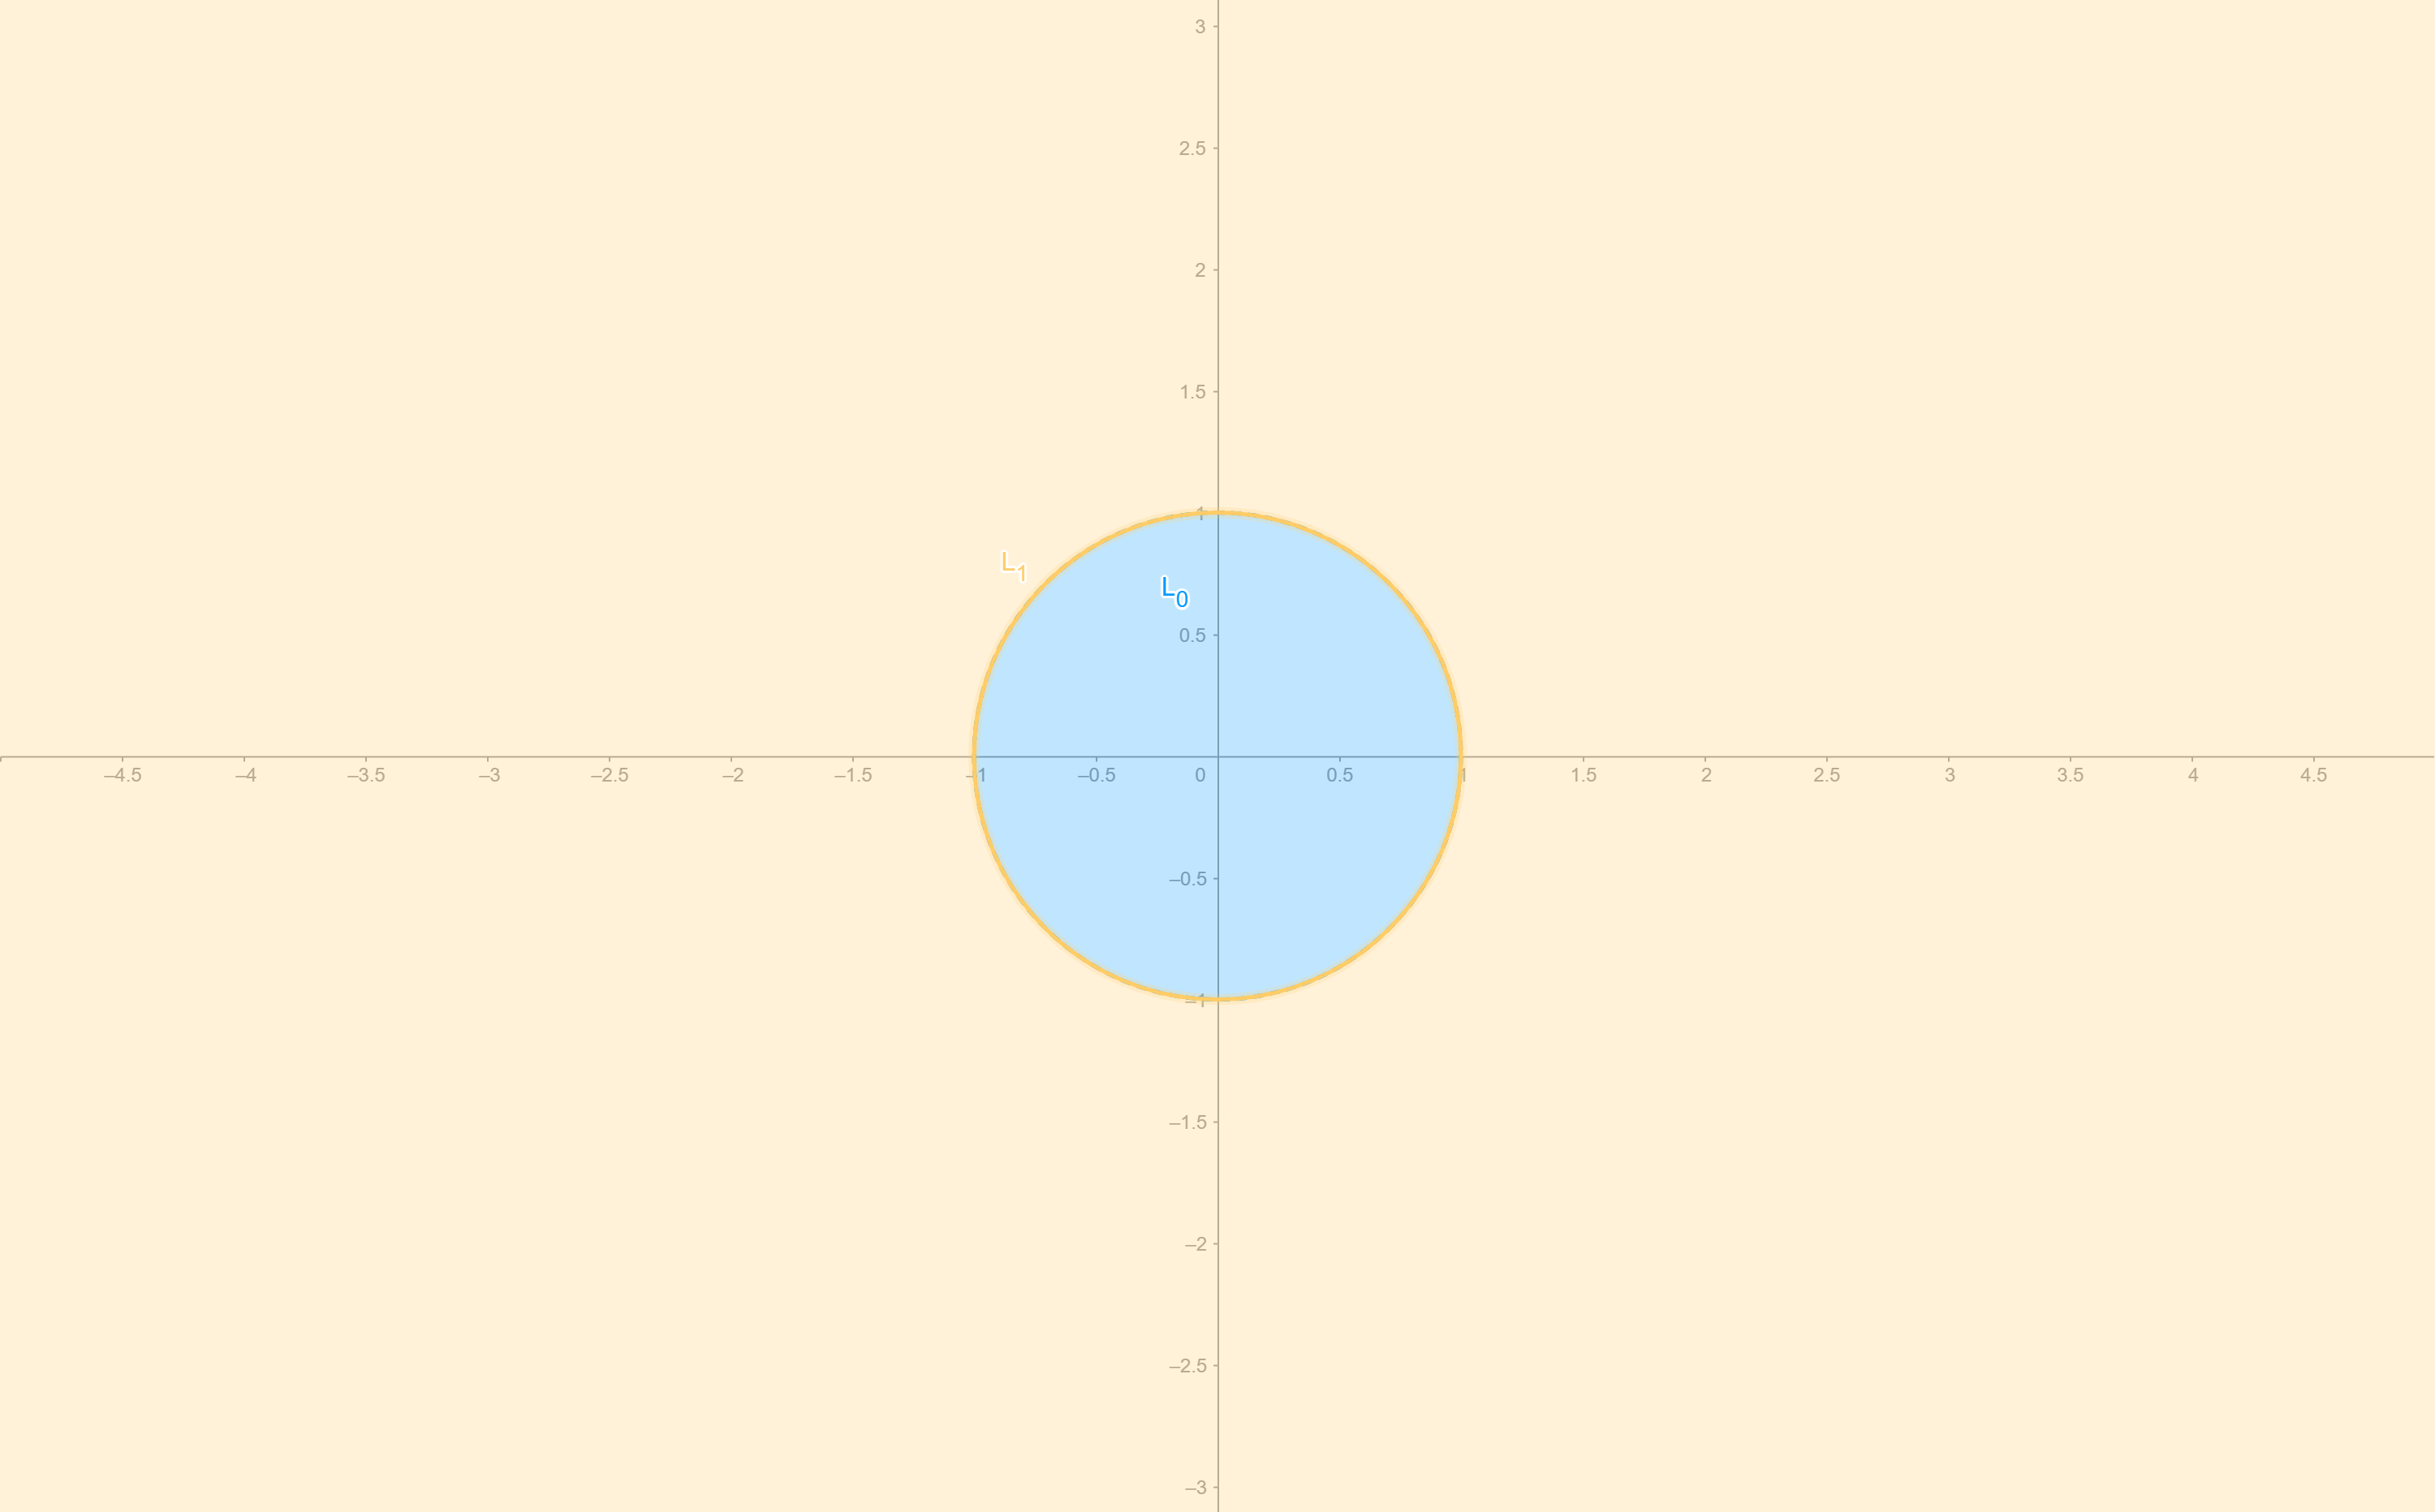
\includegraphics{Images/8.1.png}
				\centering
			\end{figure*}

			La gráfica de la función $f$ es

			\begin{figure*}[h!]
				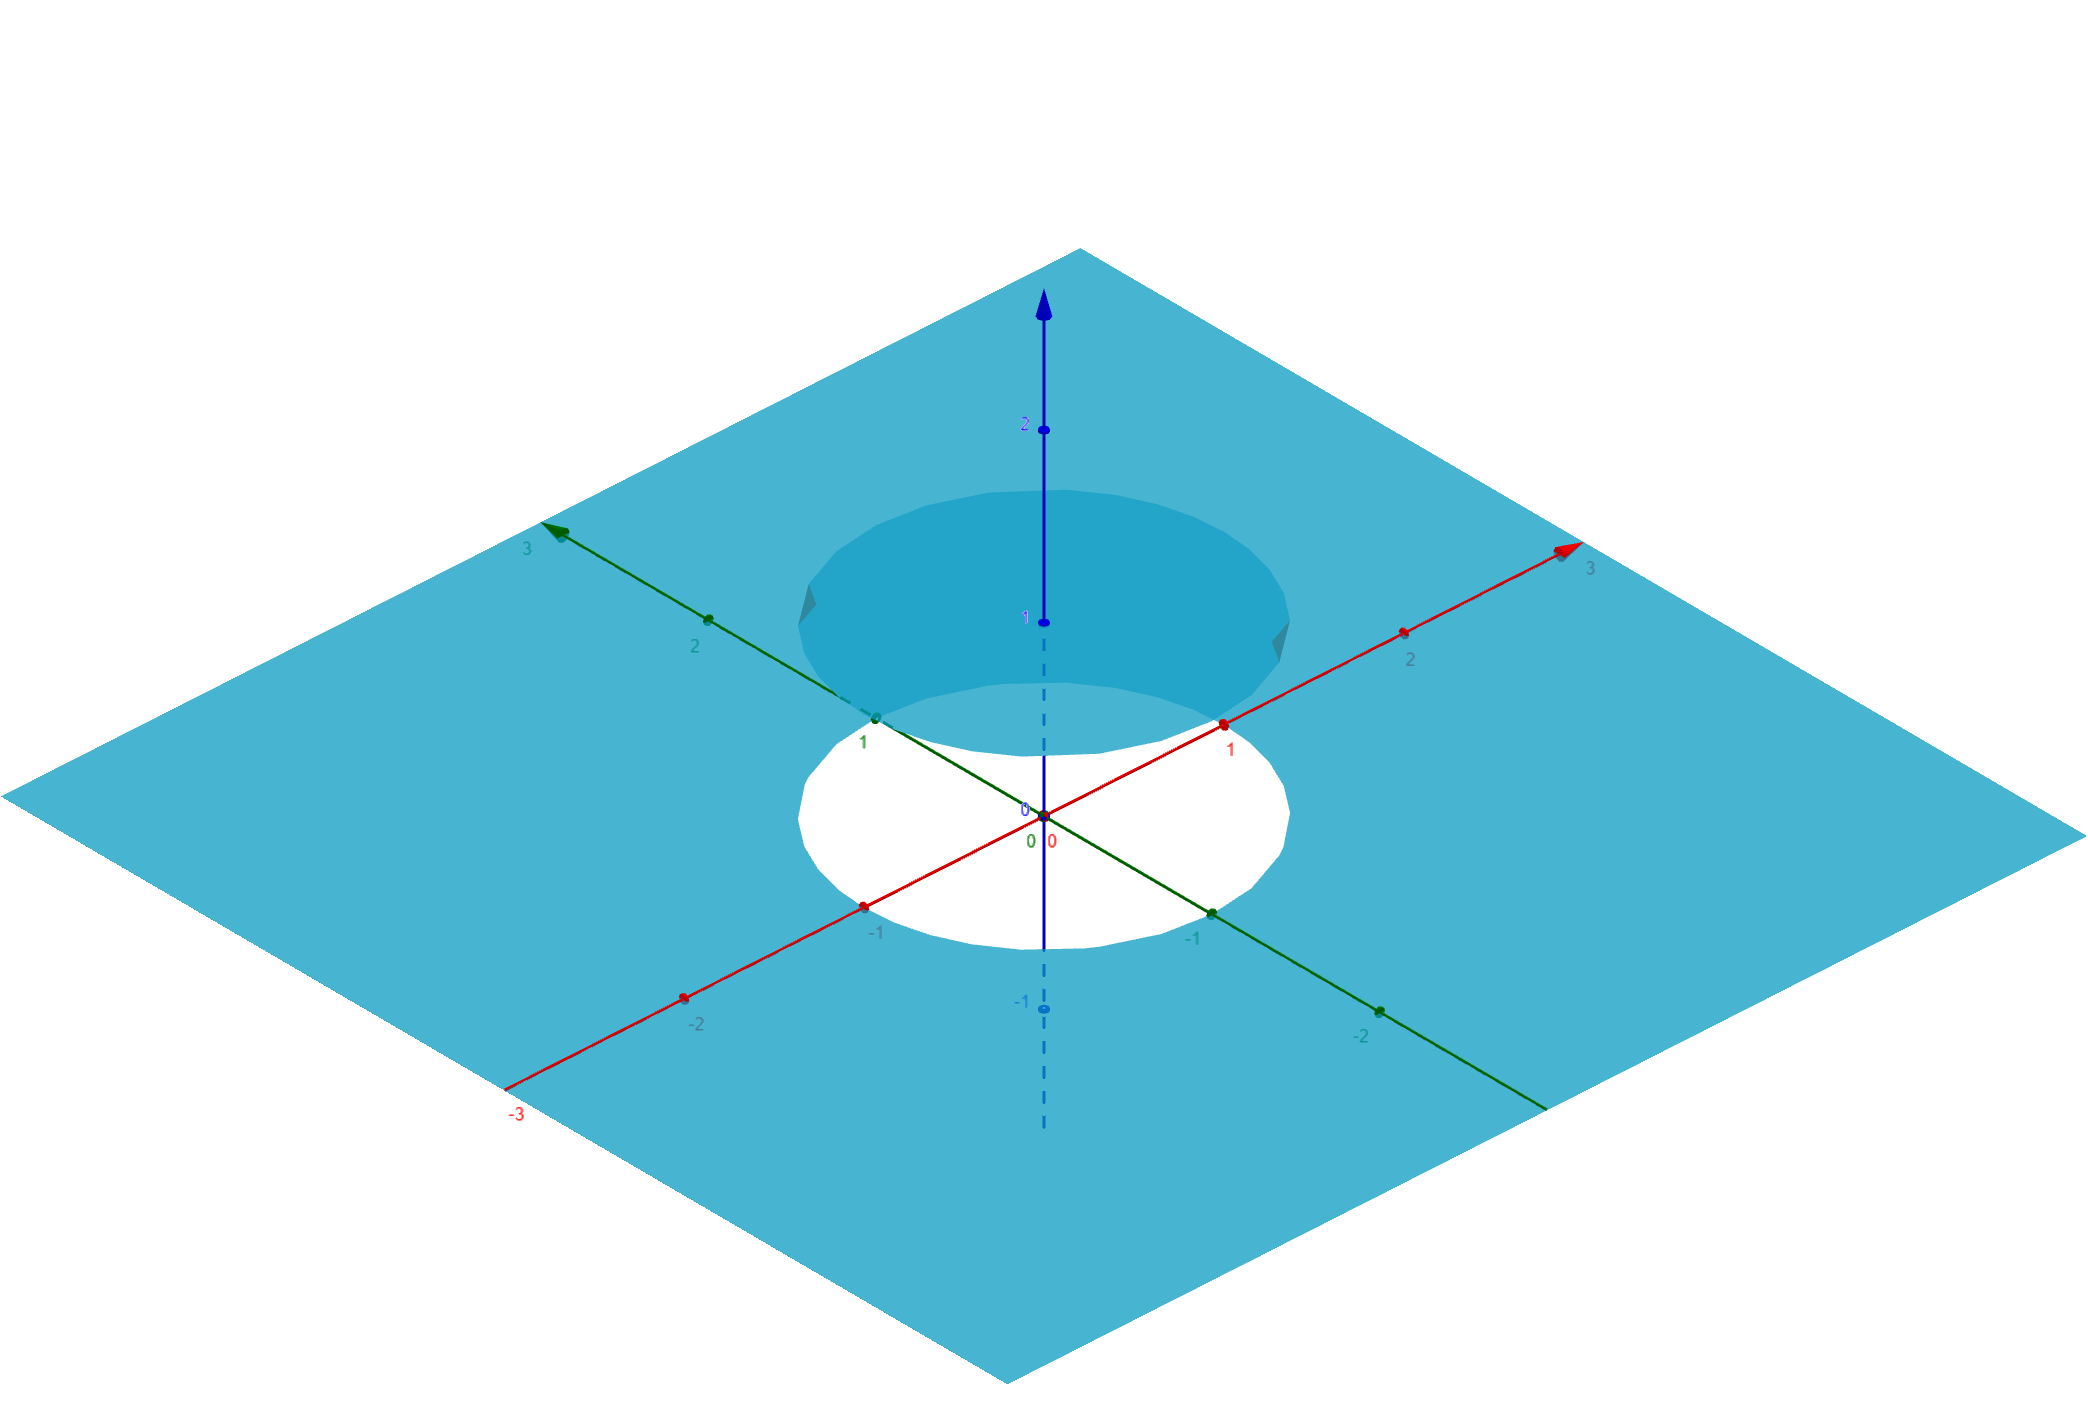
\includegraphics[scale=0.1]{Images/8.2.png}
				\centering
			\end{figure*}
		\end{sol}

		\item Sea $f(X)$ igual a $\norm{X}^2$ cuando $X$ está contenido en la bola unitaria y $0$ cuando no. Describe los conjuntos de nivel para los siguientes dominios.
		
		\begin{enumerate}
			\item $\RR$
			Los conjuntos de nivel $L_c(f)$ de $f$ solo pueden ser $c \in {0,1}$ por definición. Además por definición $f(x) = 1$ ssi $(x)$ está contenido en la bola unitaria centrada en el origen, y $f(x) = 0$ si no. Por lo tanto concluimos que

			\begin{align*}
				L_0(f) &= \set{\pars{x} | \abs{x}<1}\\
				L_1(f) &= \set{\pars{x} | \abs{x}\geq 1}
			\end{align*}

			\item $\RR^3$
			Los conjuntos de nivel $L_c(f)$ de $f$ solo pueden ser $c \in {0,1}$ por definición. Además por definición $f(x,y,z) = 1$ ssi $(x)$ está contenido en la bola unitaria centrada en el origen, y $f(x,y,z) = 0$ si no. Por lo tanto concluimos que

			\begin{align*}
				L_0(f) &= \set{\pars{x,y,z} | \norm{\pars{x,y,z}}<1}\\
				L_1(f) &= \set{\pars{x,y,z} | \norm{\pars{x,y,z}}\geq 1}
			\end{align*}

			\item $\RR^5$
			Los conjuntos de nivel $L_c(f)$ de $f$ solo pueden ser $c \in {0,1}$ por definición. Además por definición $f(x_1,x_2,x_3,x_4,x_5) = 1$ ssi $(x)$ está contenido en la bola unitaria centrada en el origen, y $f(x_1,x_2,x_3,x_4,x_5) = 0$ si no. Por lo tanto concluimos que

			\begin{align*}
				L_0(f) &= \set{\pars{x_1,x_2,x_3,x_4,x_5} | \norm{\pars{x_1,x_2,x_3,x_4,x_5}}<1}\\
				L_1(f) &= \set{\pars{x_1,x_2,x_3,x_4,x_5} | \norm{\pars{x_1,x_2,x_3,x_4,x_5}}\geq 1}
			\end{align*}
		\end{enumerate}
		\item Sea $f(X) = \norm{X}^2$, $X\in \RR^4$. Sea $A\in \RR^4$ and define
		
		\[g_A(X) = \norm{A}^2 + 2\inprod{A,X-A}.\]

		\begin{enumerate}
			\item Sea $U=X-A$. Usa la formula
			\[\norm{A+U}=\norm{A}^2+2\inprod{A,U}+\norm{U}^2\]
			para demostrar que la diferencia entre $f(X)$ y $g_a(X)$ es $\norm{U}^2$.
			\begin{proof}
				Veamos que por la formula mencionada obtenemos

				\begin{align*}
					f(X) - g_A(X) &= \norm{X}^2 - \pars{\norm{A}^2 + 2\inprod{A,X-A}}\\
					&= \norm{X}^2 - \pars{\norm{A}^2 + 2\inprod{A,U} +\norm{U}^2} + \norm{U}^2\\
					&= \norm{X}^2 - \norm{A+U} + \norm{U}^2\\
					&= \norm{U}^2
				\end{align*}
			\end{proof}
			\item Demuestra que la diferencia entre $f(X)$ y $g_a(X)$ no excede $10^{-4}$ cuando $\norm{X-A}<10^{-2}$.
			\begin{proof}
				Puesto que $f(X) - g_A(X) = \norm{X-A}^2$ y tenemos que $\norm{X-A}<10^{-2}$, al ser el cuadrado una función montona creciente concluimos que

				\[f(X) - g_A(X) < 10^{-4}.\]
			\end{proof}
		\end{enumerate}

		\newpage
		\item Describe y haz un bosquejo de los conjuntos de nivel $c$ ($f(x,y)=c$ en $\RR^2$), para las siguientes funciones $f$ y valores $c$. Ayudate de estos conjuntos de nivel para hacer un bosquejo de la gráfica de la función.
		\begin{enumerate}
			\item $f(x,y)=x+2y, c=-1,0,1,2$
			
			Si $f(x,y)=c$ entonces obtenemos que

			\[y = -\frac{x}{2} + \frac{c}{2},\]

			la cuál es la ecuación de la recta con pendiente $-\frac{1}{2}$ y cruce con el eje $y$ en $\frac{c}{2}$. Con ello vemos que

			\begin{align*}
				L_{-1}(f) &= \set{(x,y) | y = -\frac{x}{2} - \frac{1}{2}}\\
				L_{0}(f) &= \set{(x,y) | y = -\frac{x}{2}}\\
				L_{1}(f) &= \set{(x,y) | y = -\frac{x}{2} + \frac{1}{2}}\\
				L_{2}(f) &= \set{(x,y) | y = -\frac{x}{2} + 1}\\
			\end{align*}

			Cuyas gráficas son

			\begin{figure*}[h!]
				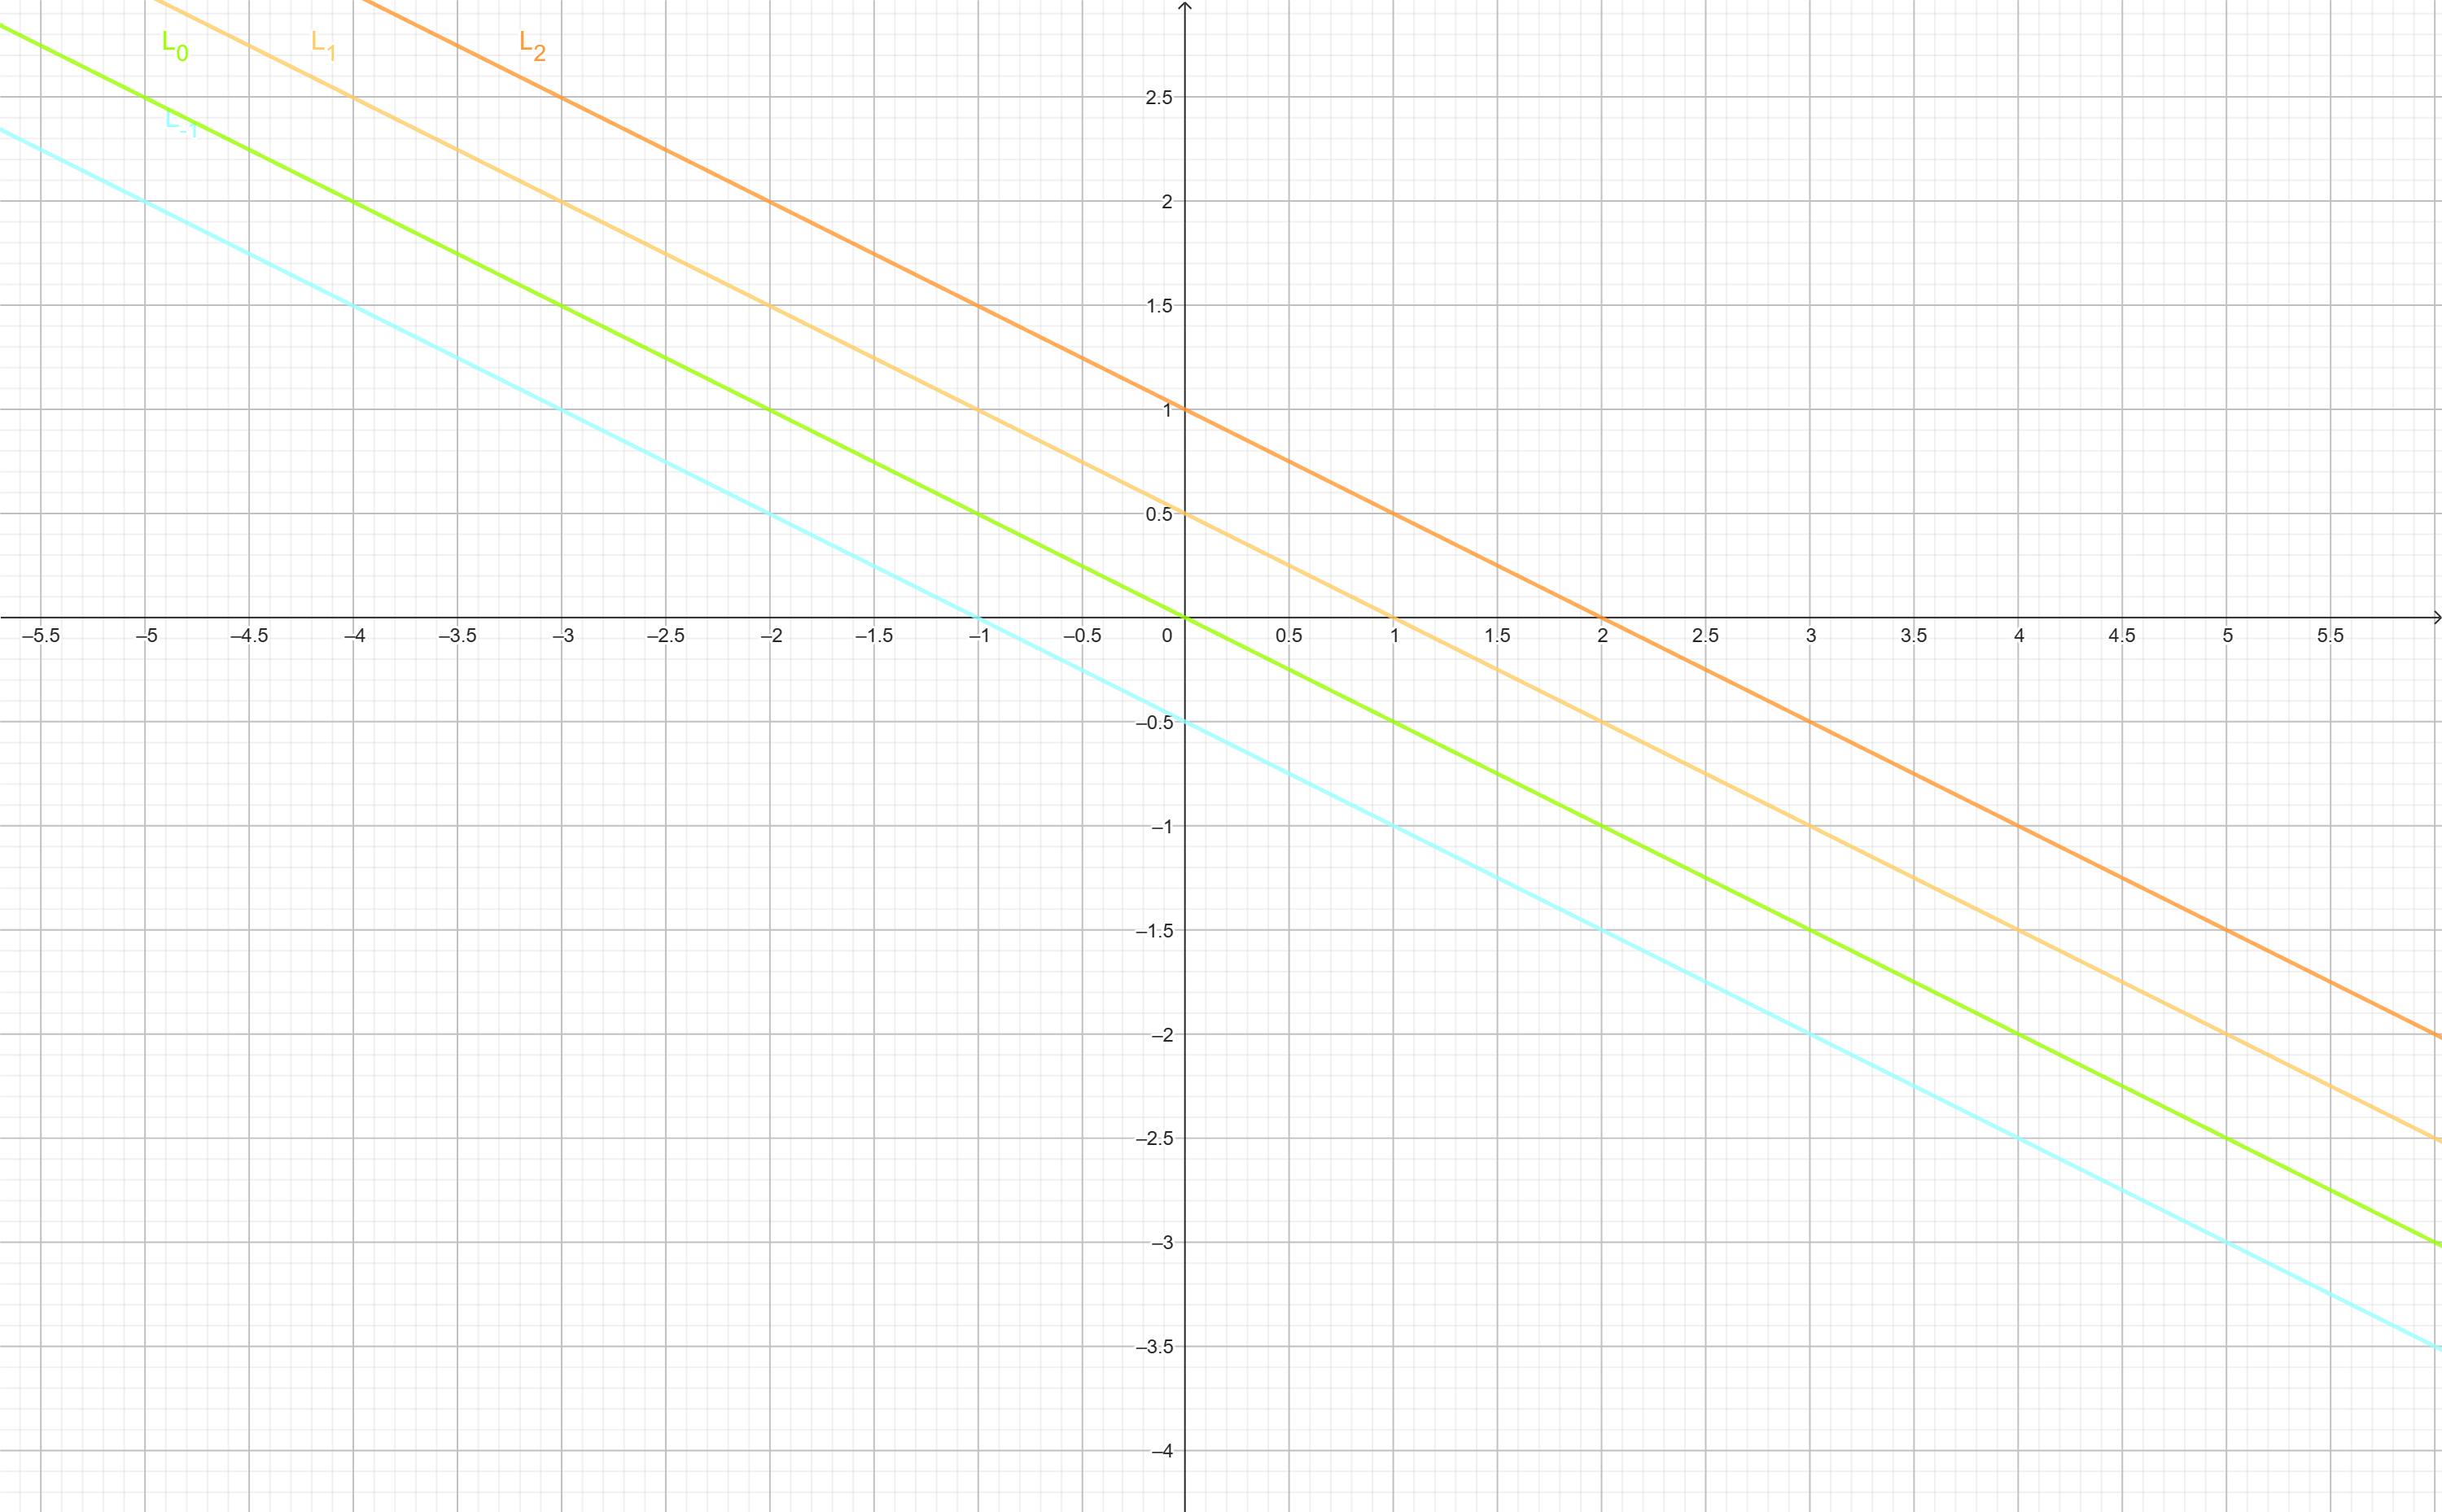
\includegraphics[scale=0.8]{Images/10.1.1.png}
				\centering
			\end{figure*}

			Con ello obtenemos la gráfica de la función $f$

			\begin{figure*}[h!]
				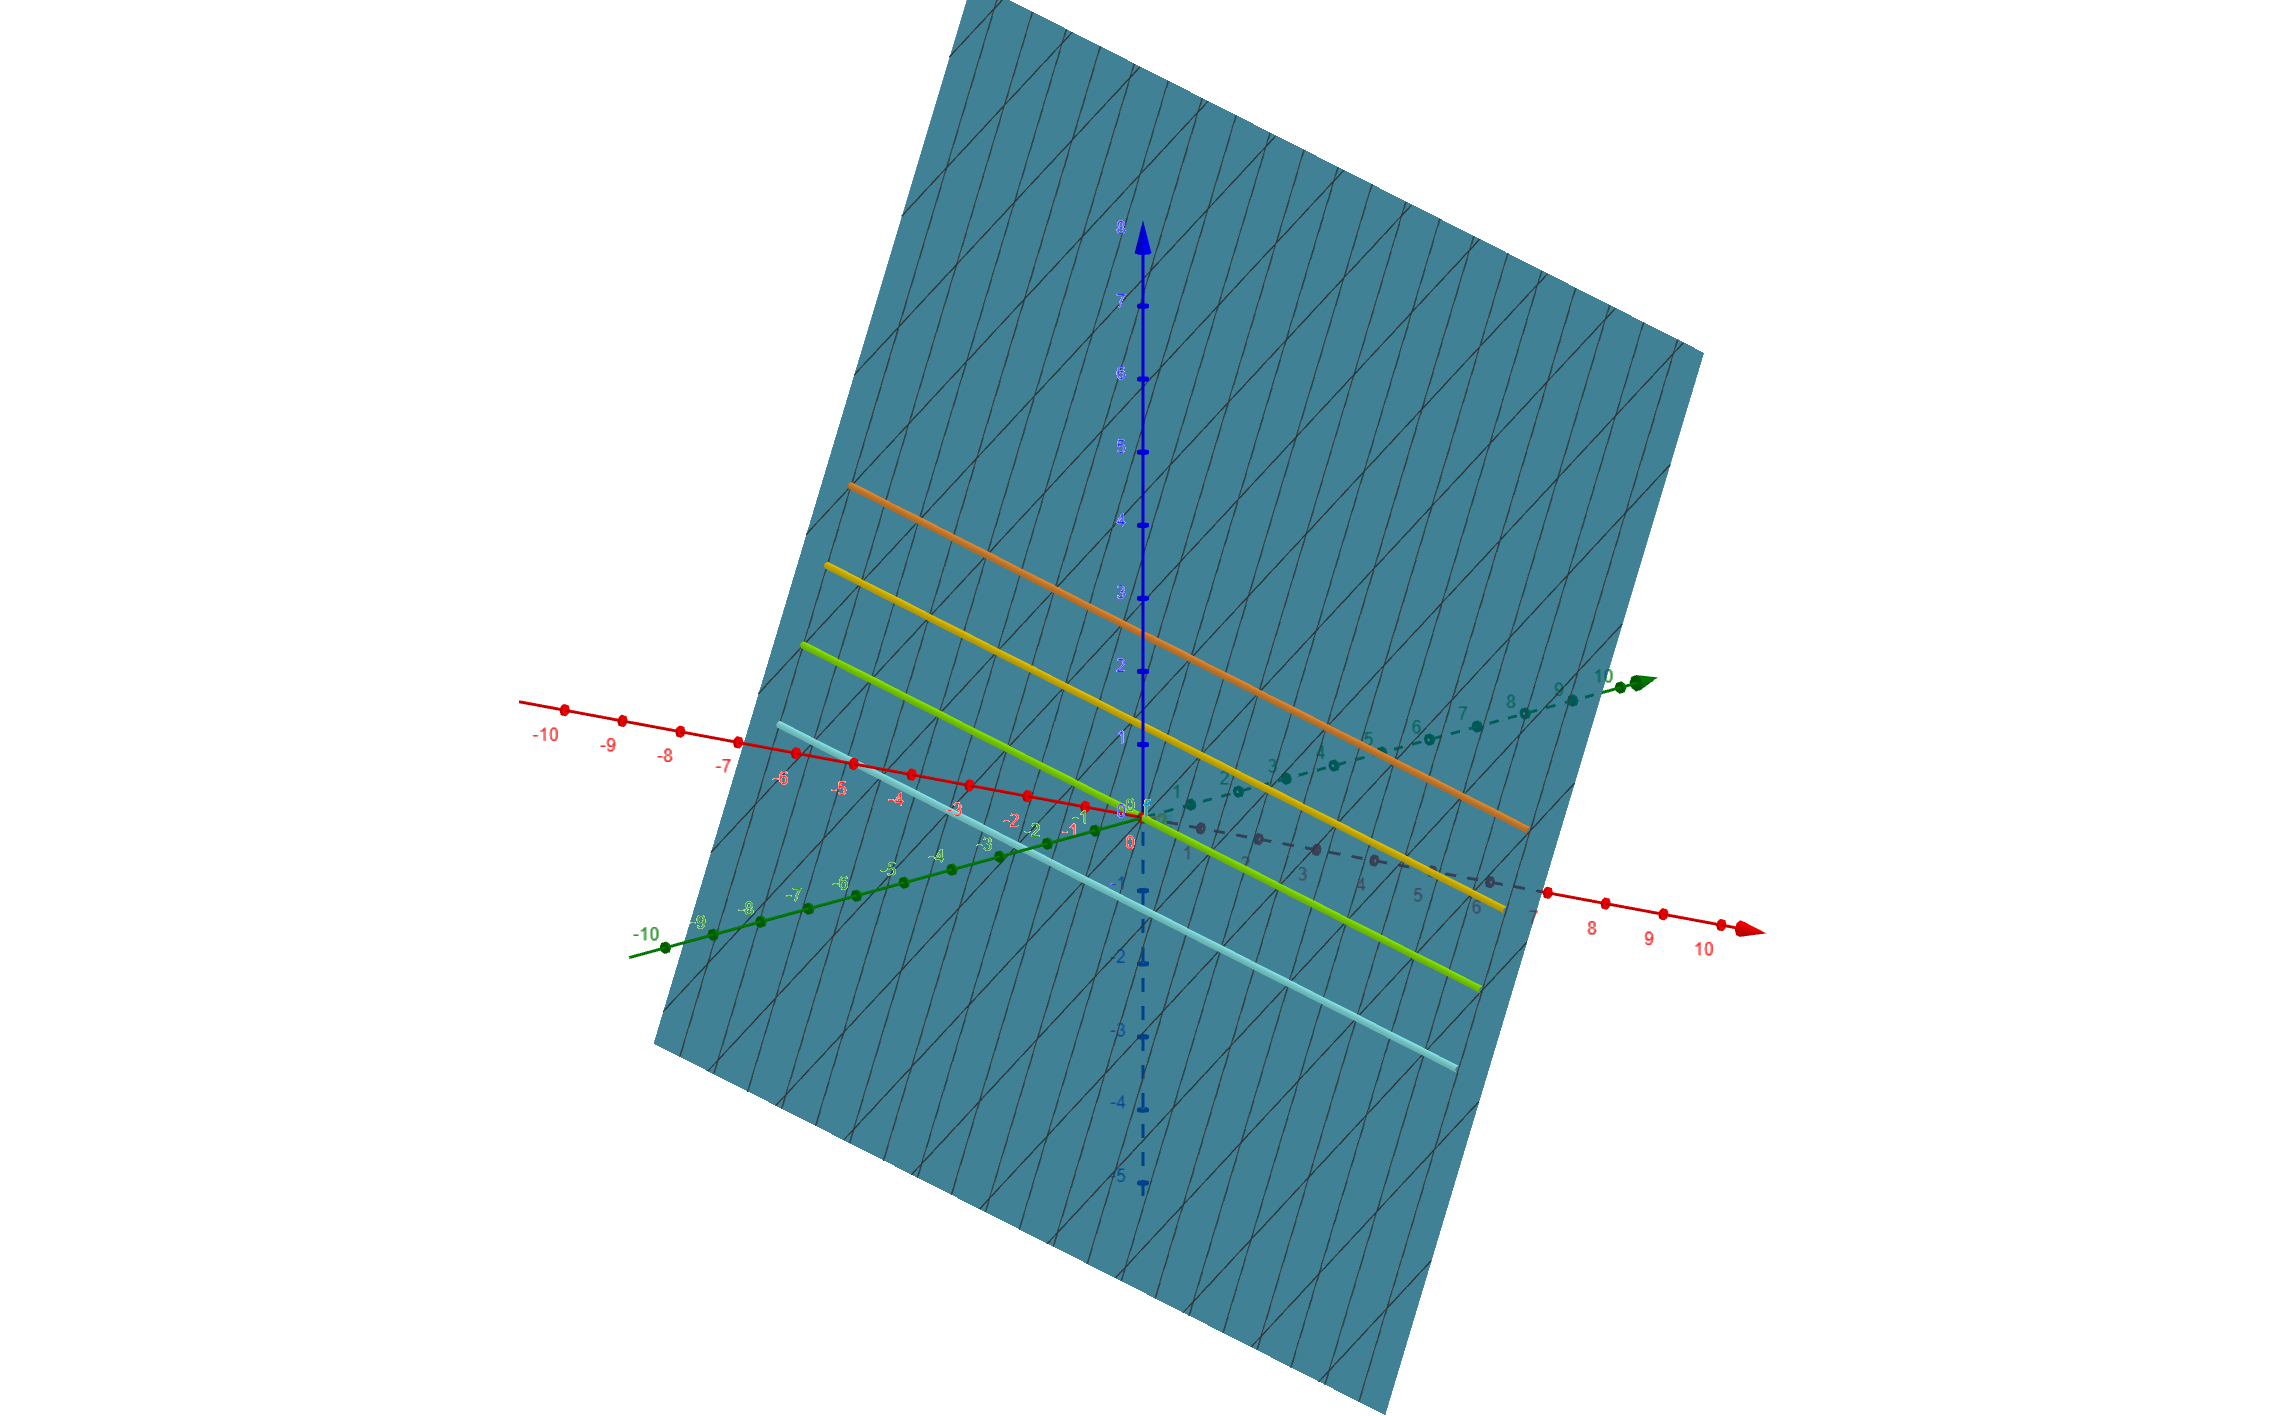
\includegraphics[scale=0.1]{Images/10.1.2.png}
				\centering
			\end{figure*}

			\newpage

			\item $f(x,y)=xy, c=-1,0,1,2$
			
			Si $f(x,y)=c$ entonces obtenemos que

			\[y = c/x,\]

			la cuál es la ecuación de una hiperbola rotada 45 grados, con eje mayor $y=x$ cuando $c>0$ y $y=-x$ cuando $c < 0$. Con ello veamos que

			\begin{align*}
				L_{-1}(f) &= \set{(x,y) | y = -\frac{1}{x}}\\
				L_{0}(f) &= \set{(x,y) | y = 0}\\
				L_{1}(f) &= \set{(x,y) | y = \frac{1}{x}}\\
				L_{2}(f) &= \set{(x,y) | y = \frac{2}{x}}\\
			\end{align*}

			Cuyas gráficas son

			\begin{figure*}[h!]
				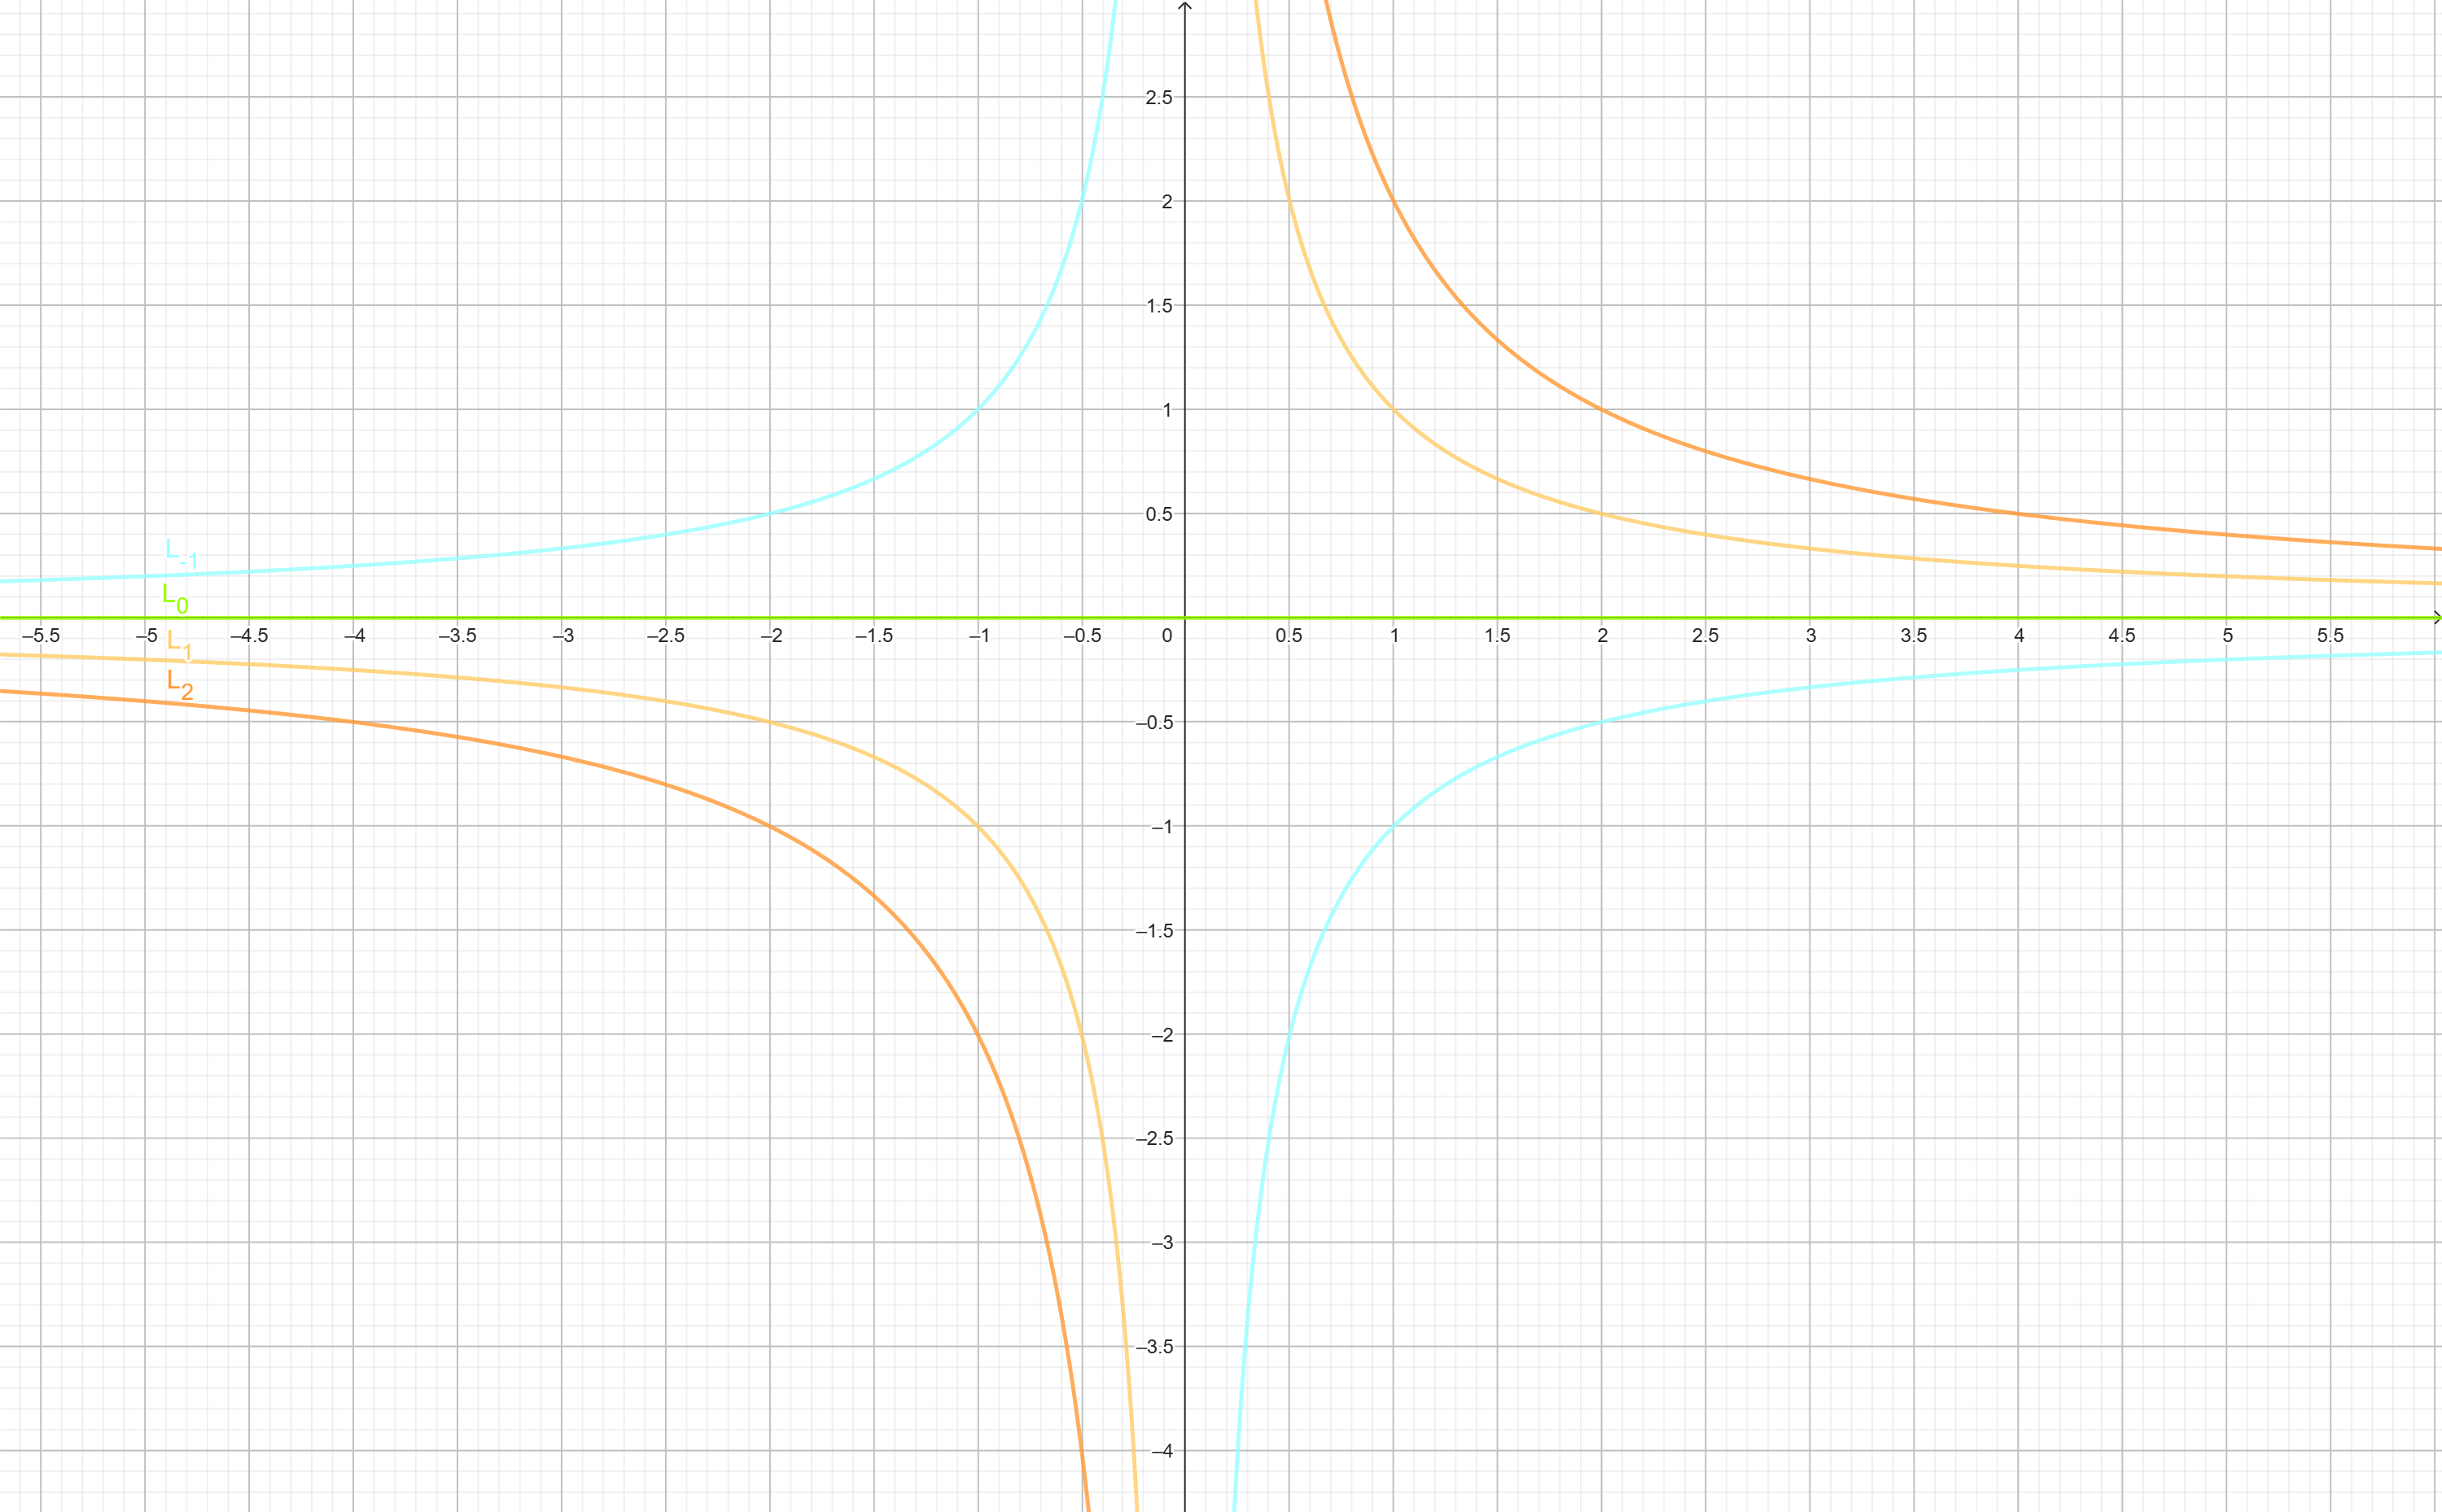
\includegraphics[scale=0.9]{Images/10.2.1.png}
				\centering
			\end{figure*}

			Con ello obtenemos la gráfica de la función $f$

			\begin{figure*}[h!]
				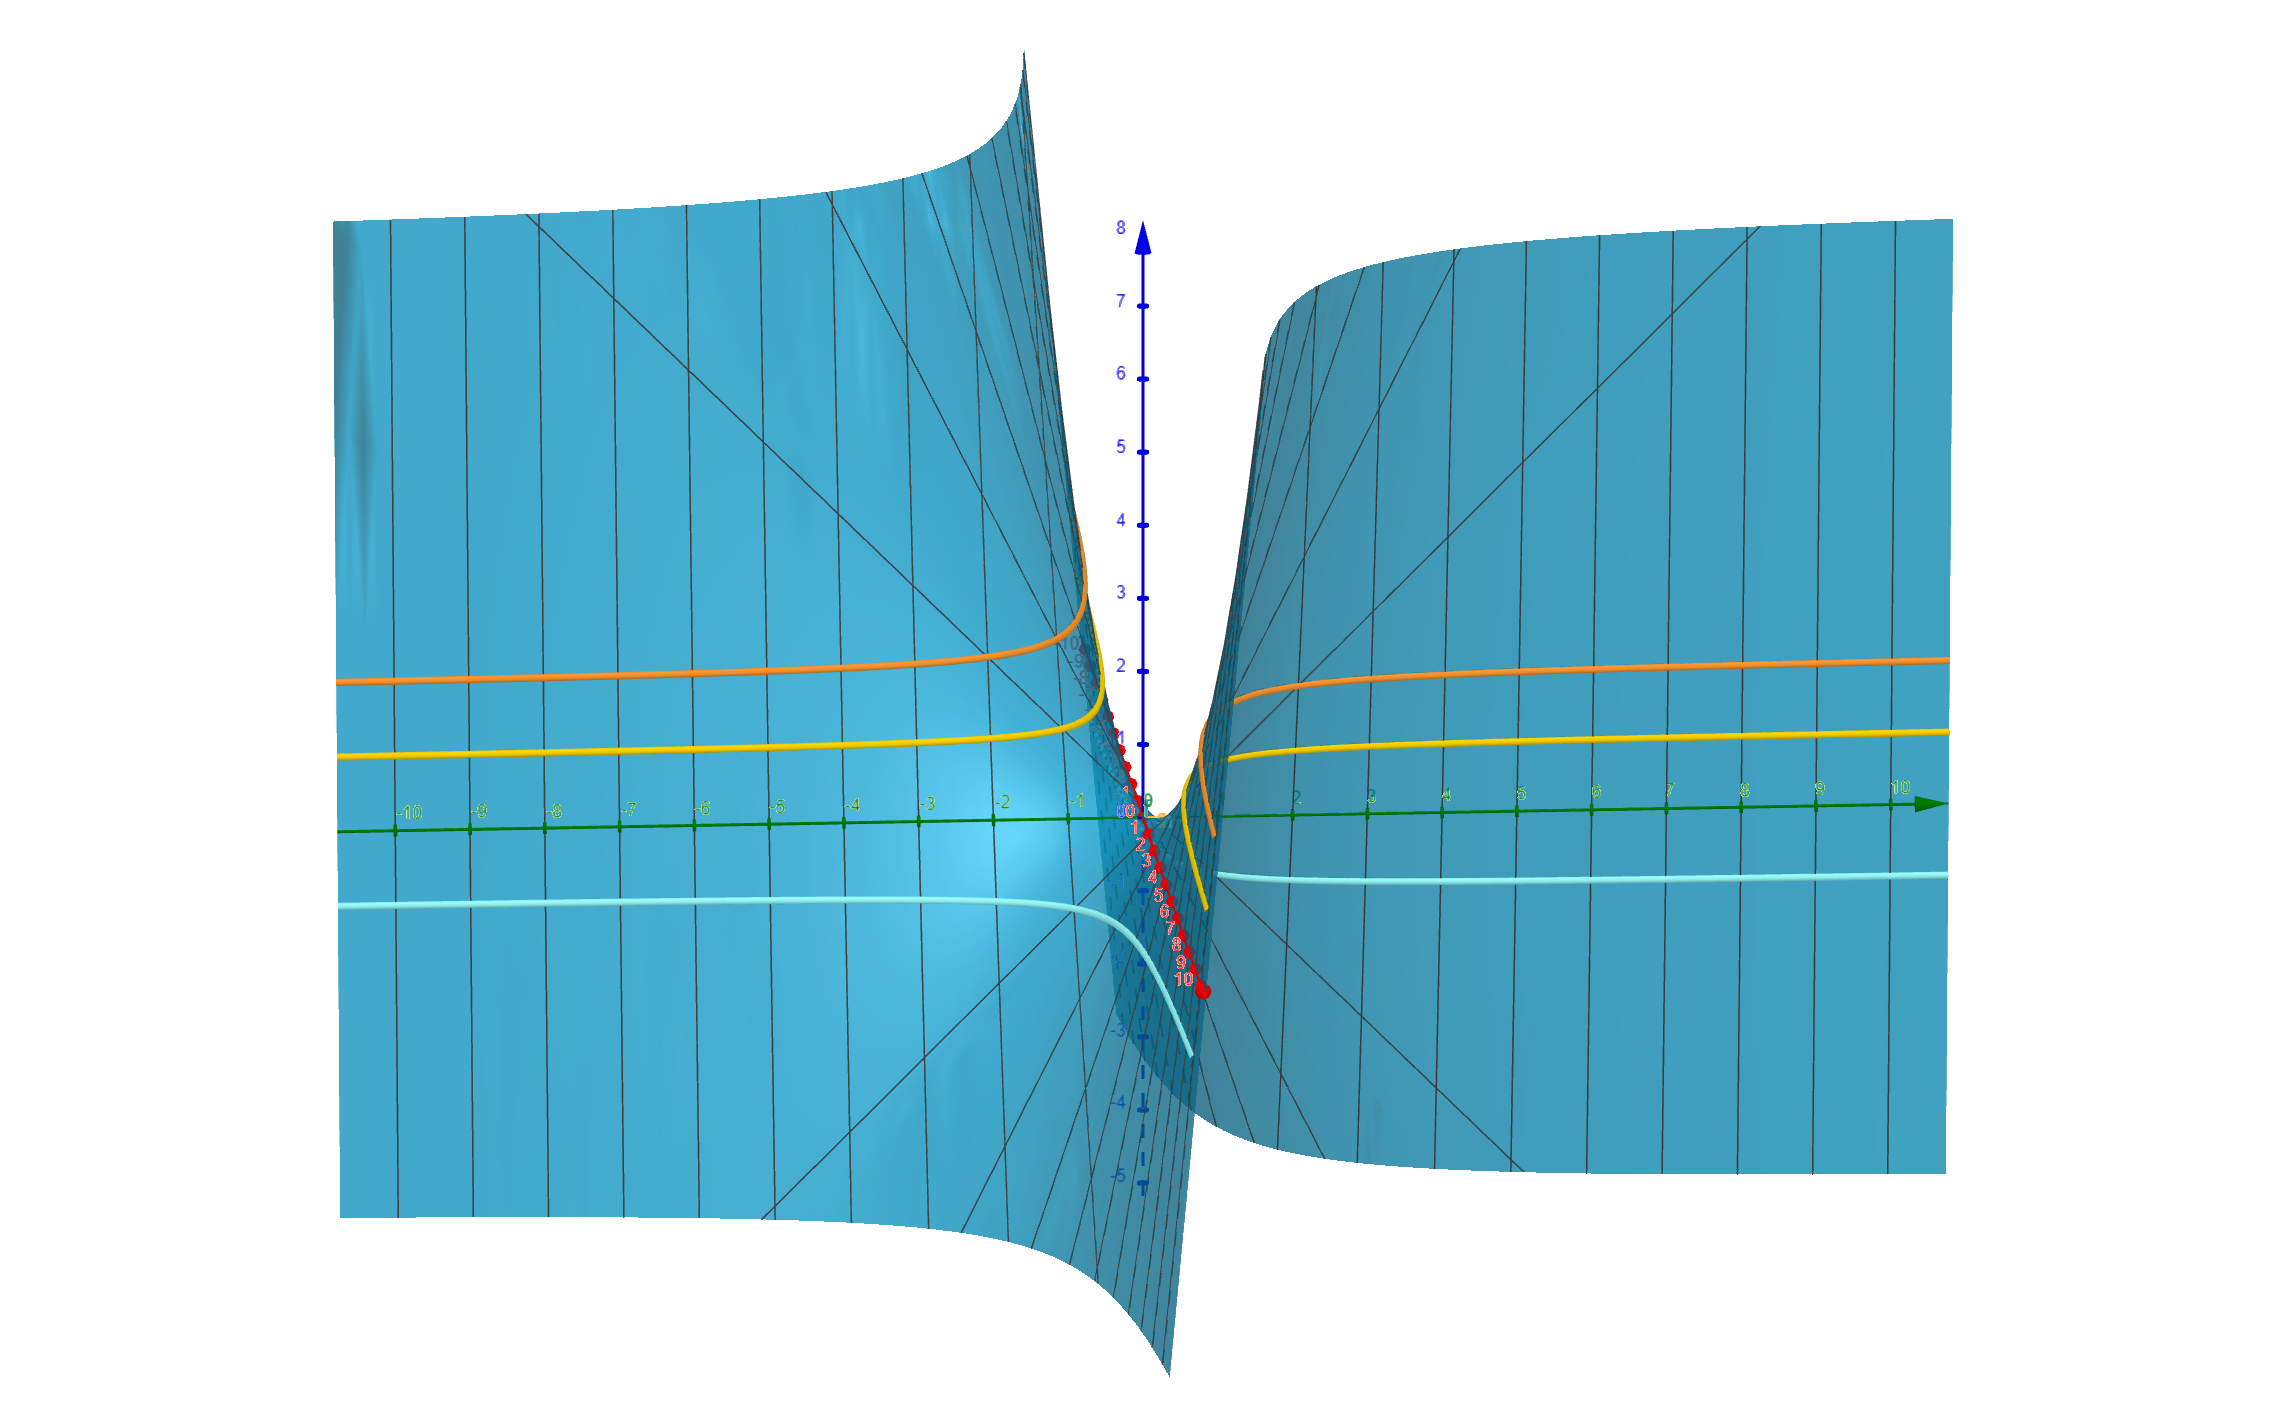
\includegraphics[scale=0.1]{Images/10.2.2.png}
				\centering
			\end{figure*}

			\newpage

			\item $f(x,y)=x^2-y, c=-1,0,1,2$
			
			Si $f(x,y)=c$ entonces obtenemos que

			\[y = x^2-c,\]

			la cuál es la ecuación de una hiperbola rotada 45 grados, con eje mayor $y=x$ cuando $c>0$ y $y=-x$ cuando $c < 0$. Con ello veamos que

			\begin{align*}
				L_{-1}(f) &= \set{(x,y) | y = x^2+1}\\
				L_{0}(f) &= \set{(x,y) | y = 0}\\
				L_{1}(f) &= \set{(x,y) | y = x^2-1}\\
				L_{2}(f) &= \set{(x,y) | y = x^2-2}\\
			\end{align*}

			Cuyas gráficas son

			\begin{figure*}[h!]
				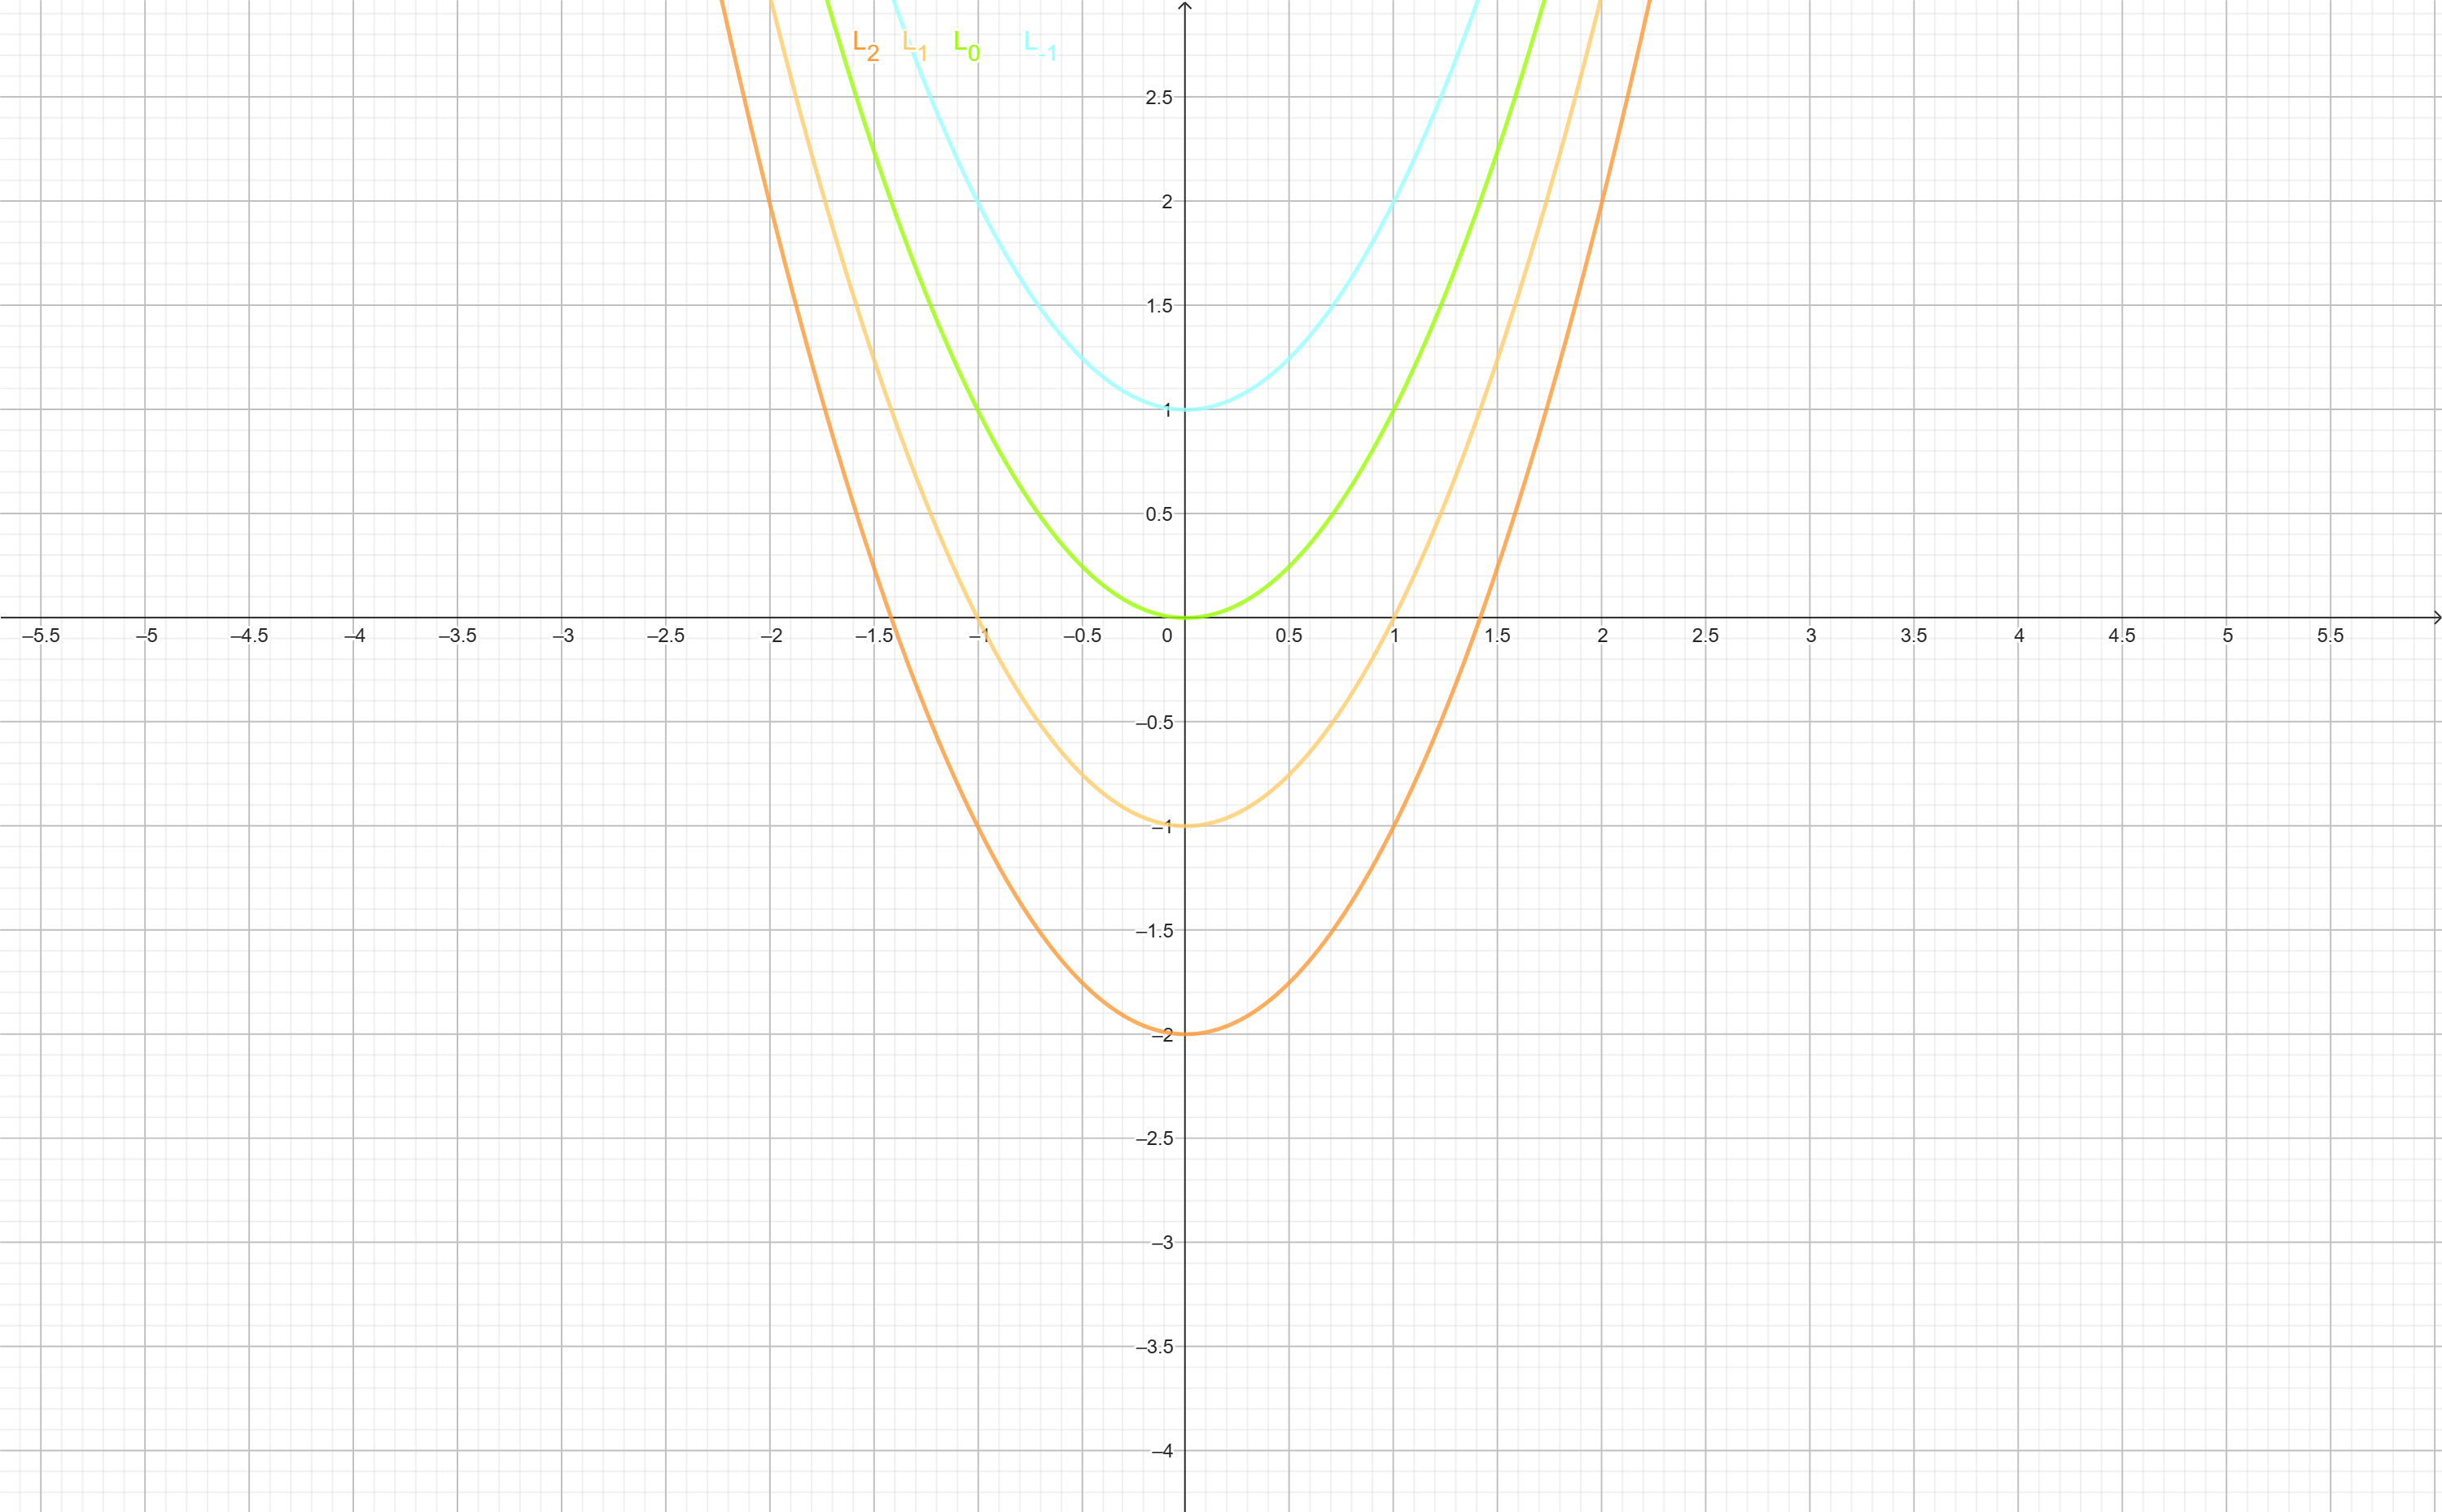
\includegraphics{Images/10.3.1.png}
				\centering
			\end{figure*}

			Con ello obtenemos la gráfica de la función $f$

			\begin{figure*}[h!]
				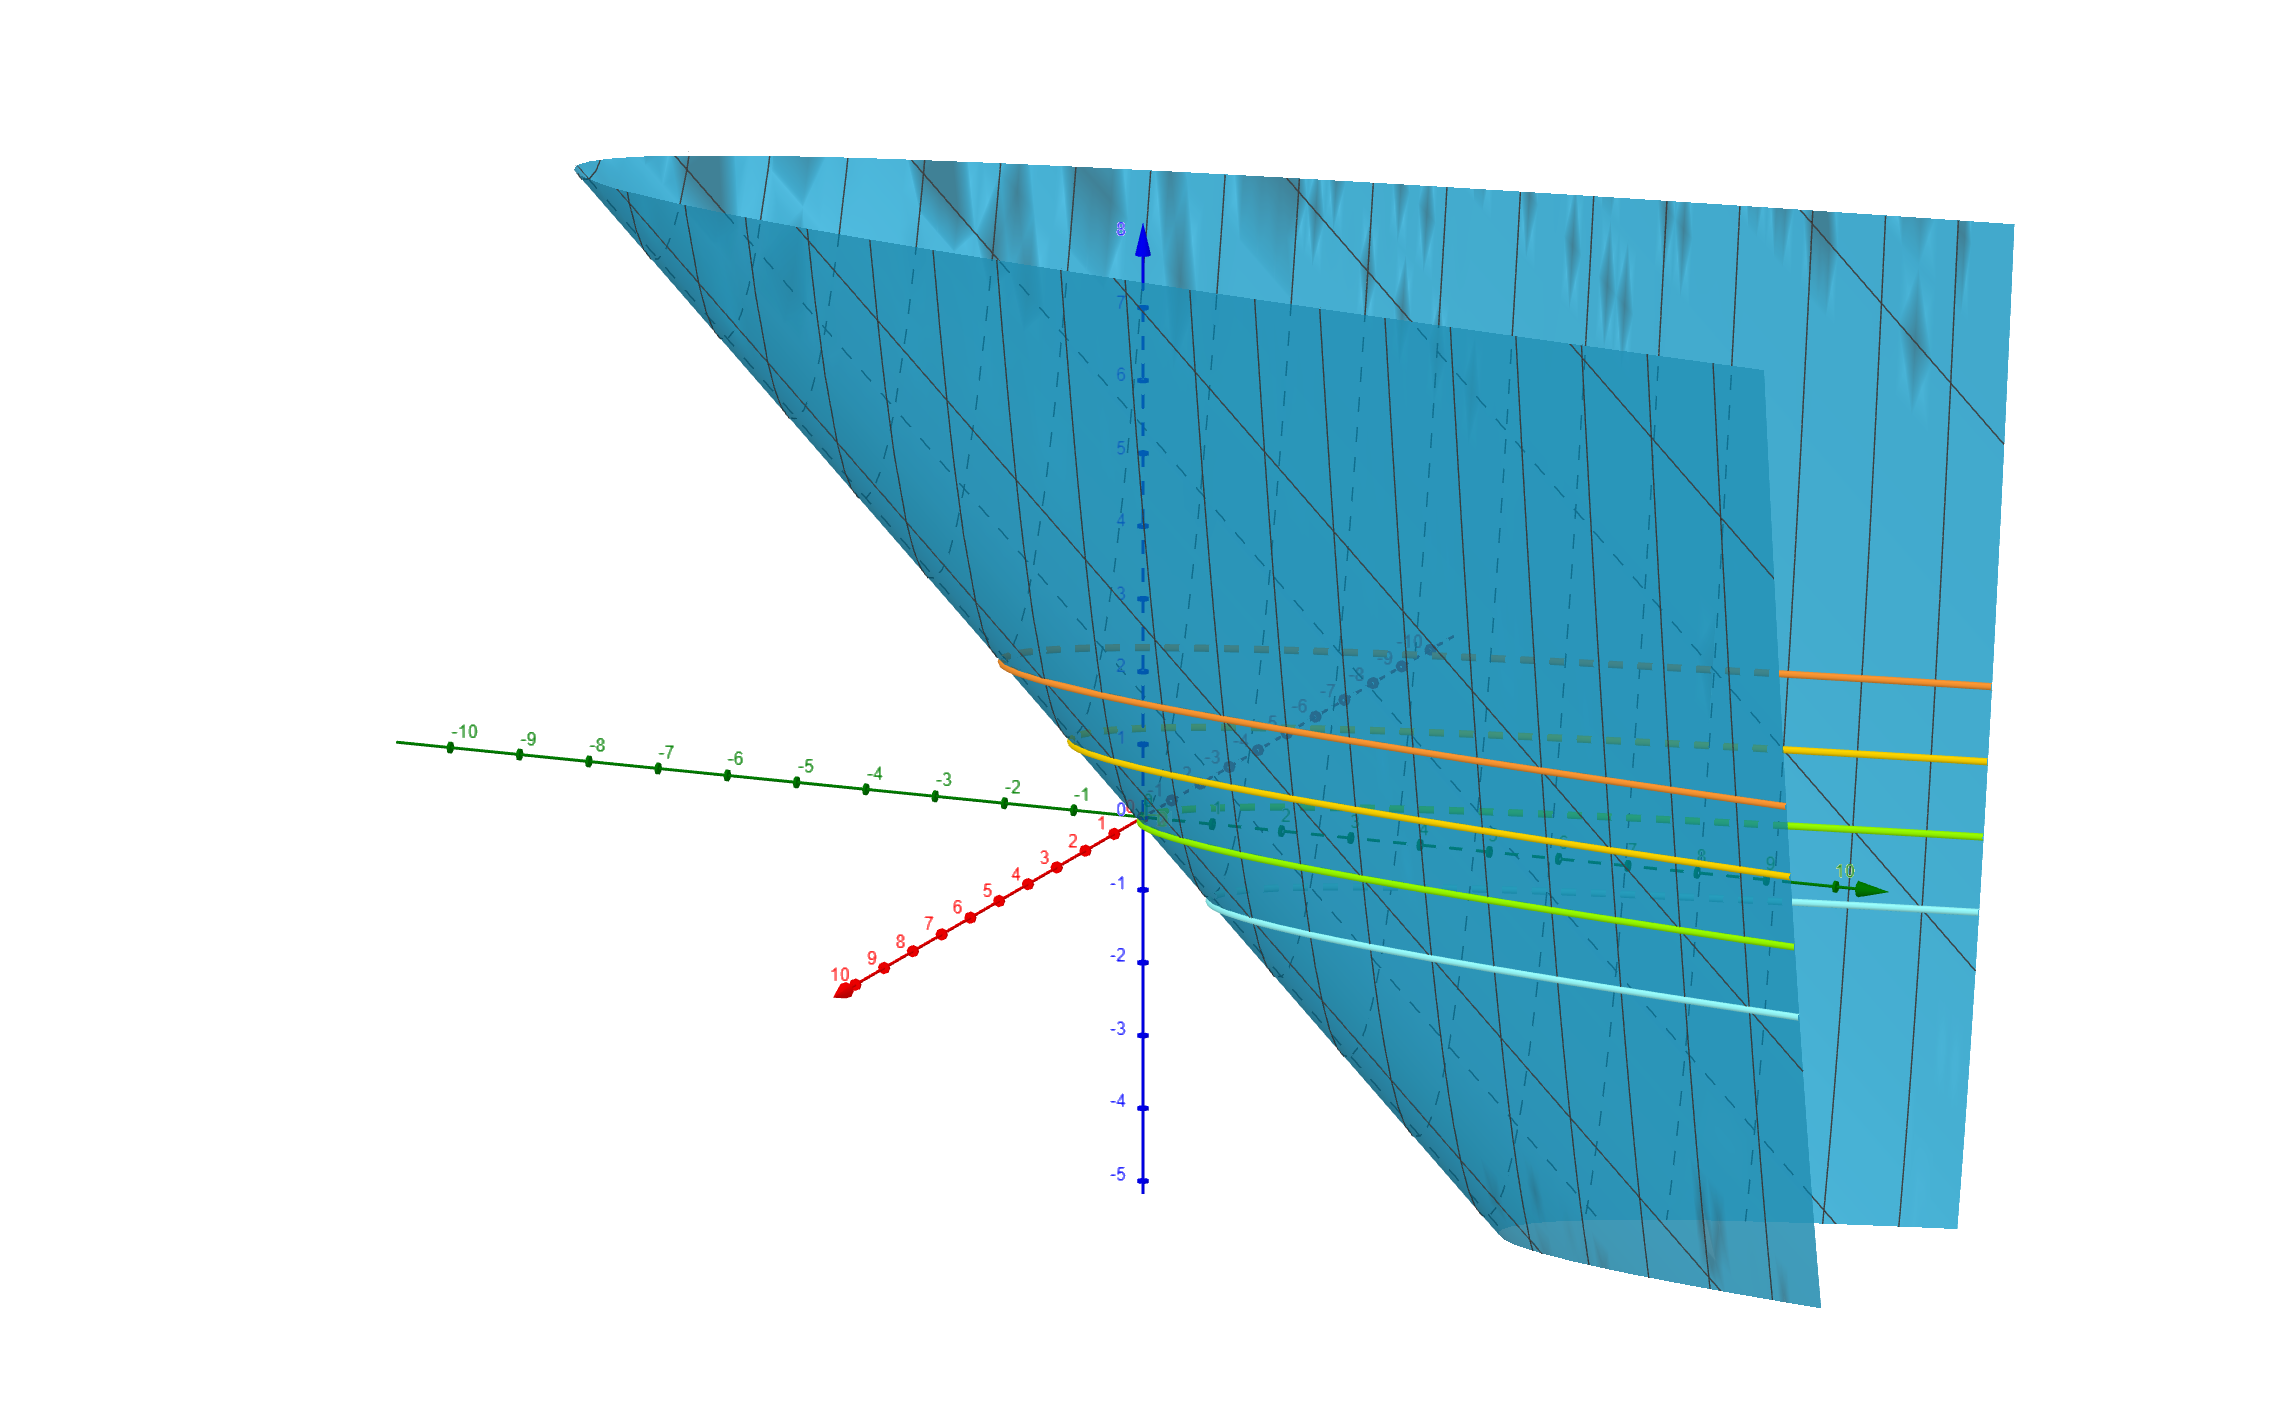
\includegraphics[scale=0.1]{Images/10.3.2.png}
				\centering
			\end{figure*}

			\newpage

			\item $f(x,y)=\sqrt{1-x^2-y^2}, c=0,\frac{1}{2},1$
			
			Si $f(x,y)=c$ entonces obtenemos que

			\[y = \sqrt{1-x^2-c^2},\]

			la cuál es la ecuación de una semicircunferencia de radio $c$ sobre el eje $x$. Con ello veamos que

			\begin{align*}
				L_{0}(f) &= \set{(x,y) | y = \sqrt{1-x^2}}\\
				L_{\frac{1}{2}}(f) &= \set{(x,y) | y = \sqrt{1-x^2-1/4}}\\
				L_{1}(f) &= \set{(x,y) | y = \sqrt{-x^2}}\\
			\end{align*}

			Cuyas gráficas son

			\begin{figure*}[h!]
				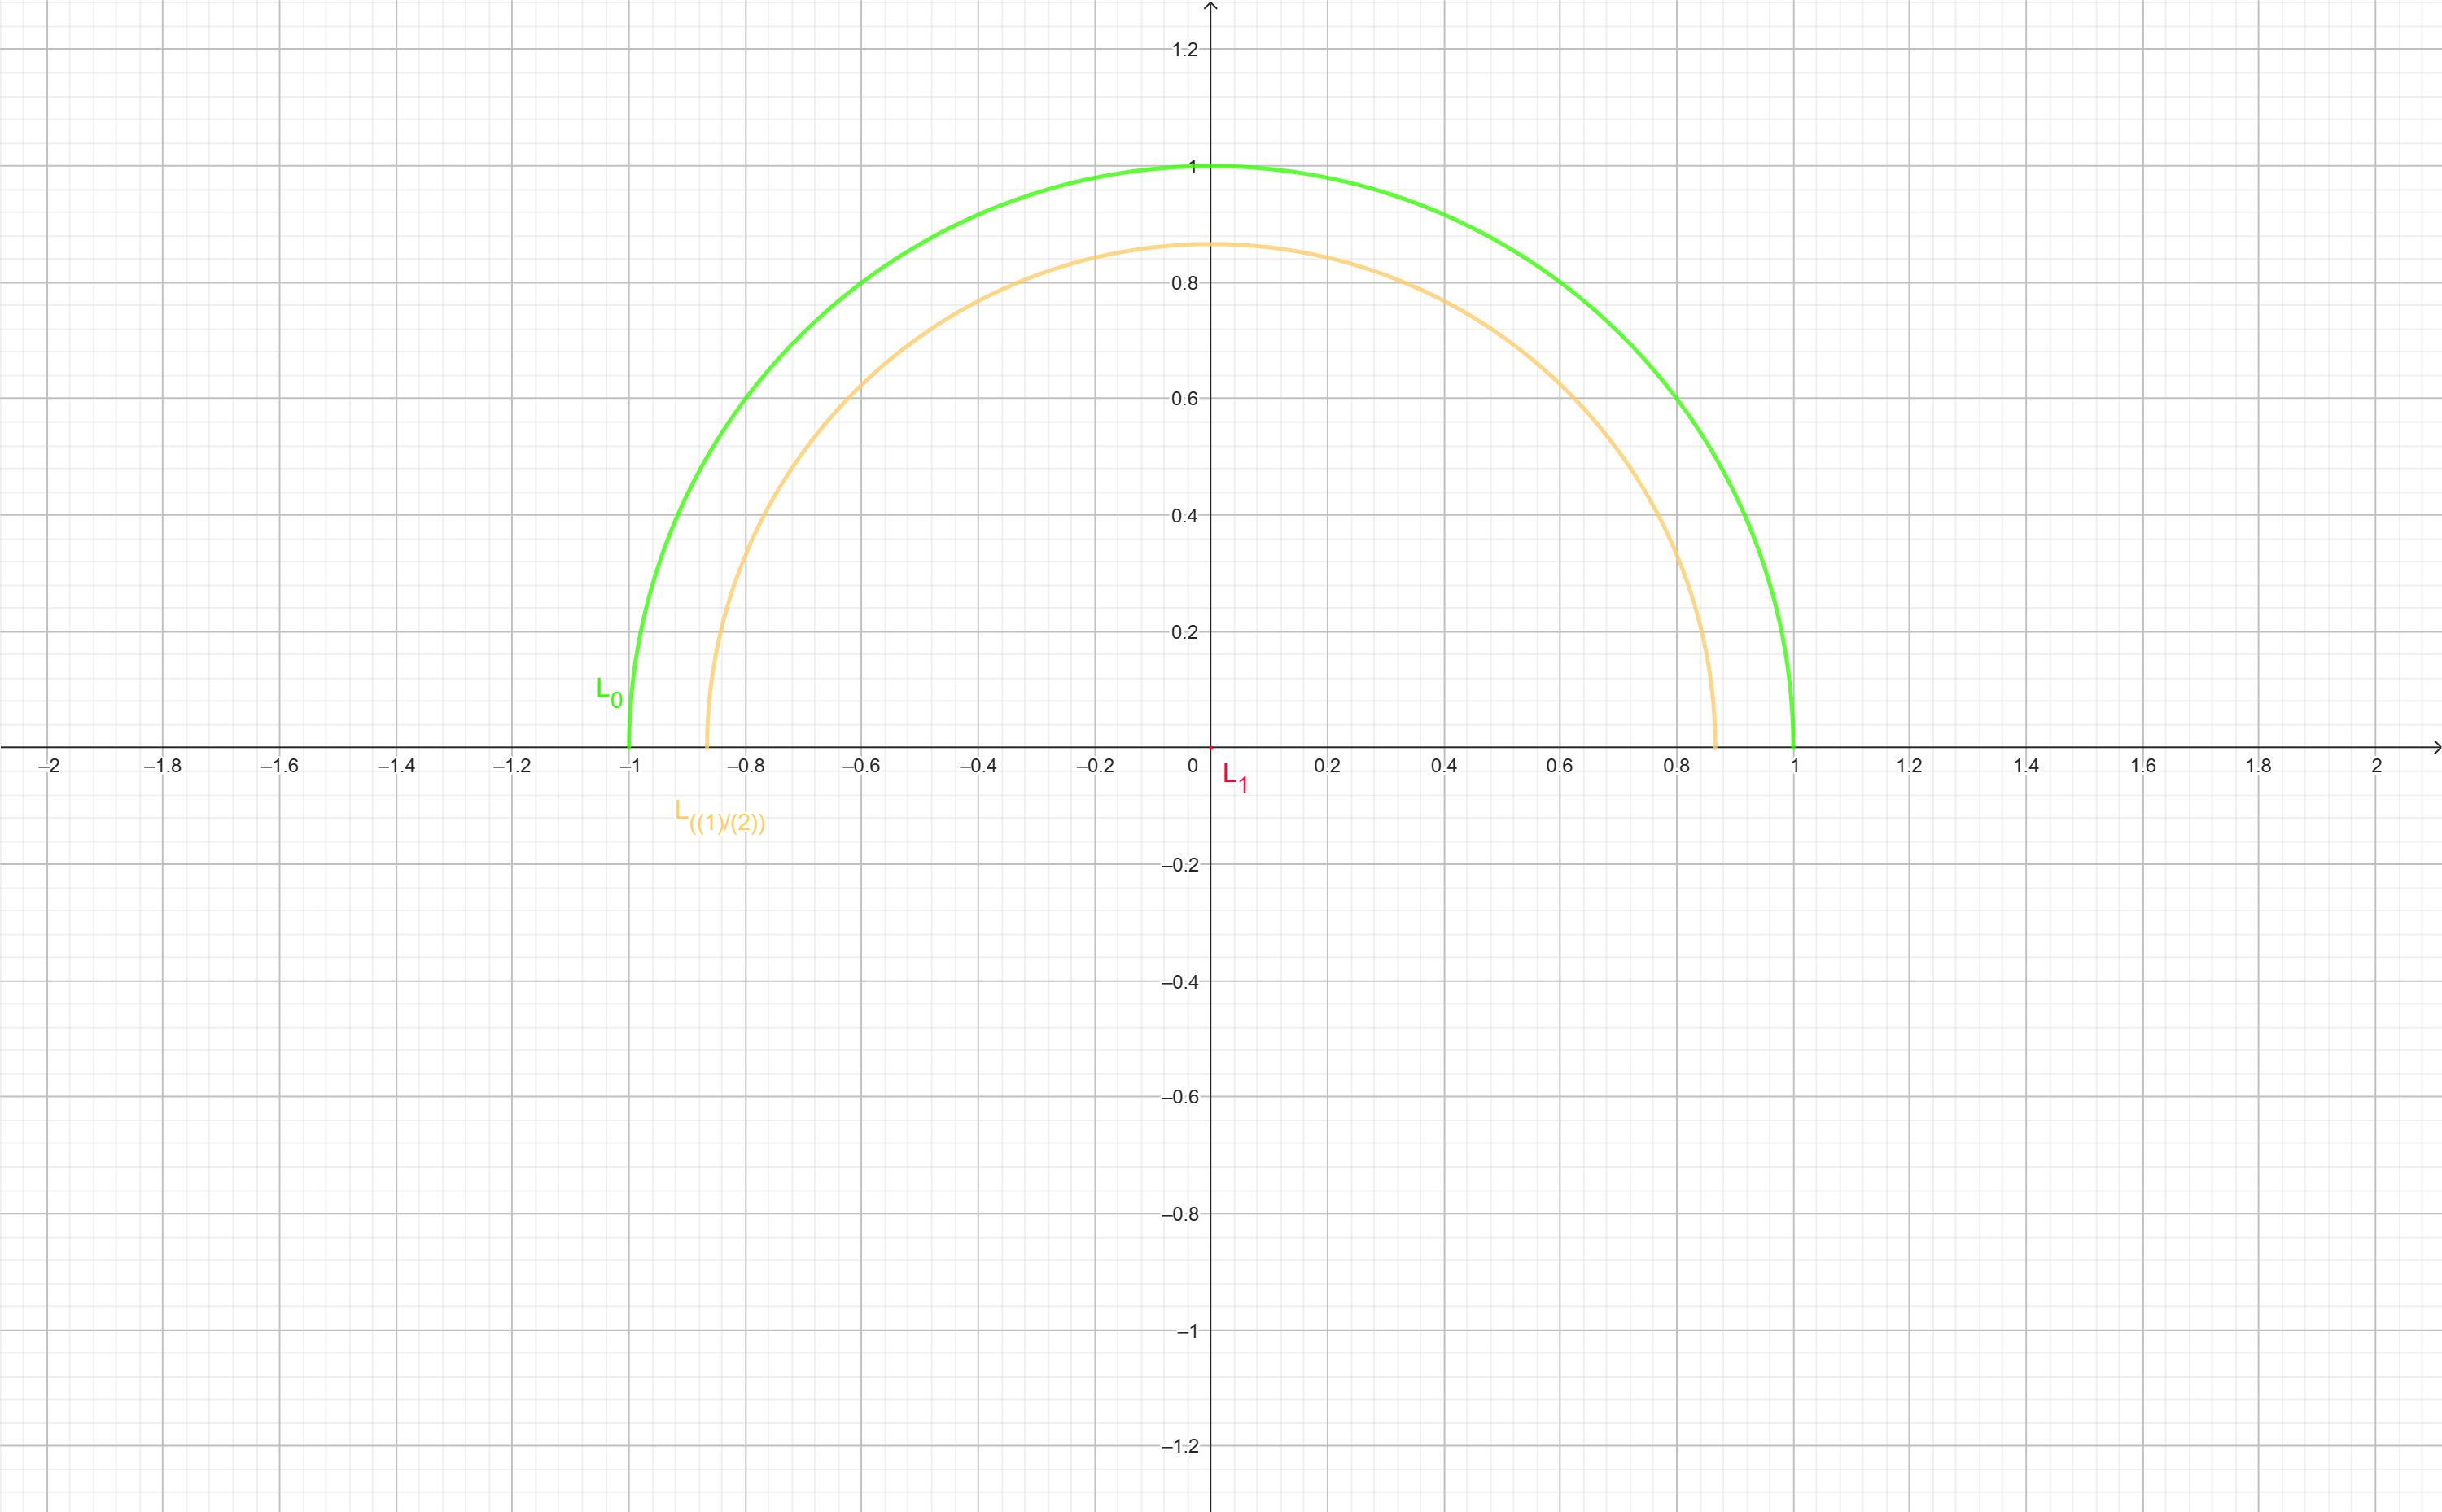
\includegraphics{Images/10.4.1.png}
				\centering
			\end{figure*}

			Con ello obtenemos la gráfica de la función $f$

			\begin{figure*}[h!]
				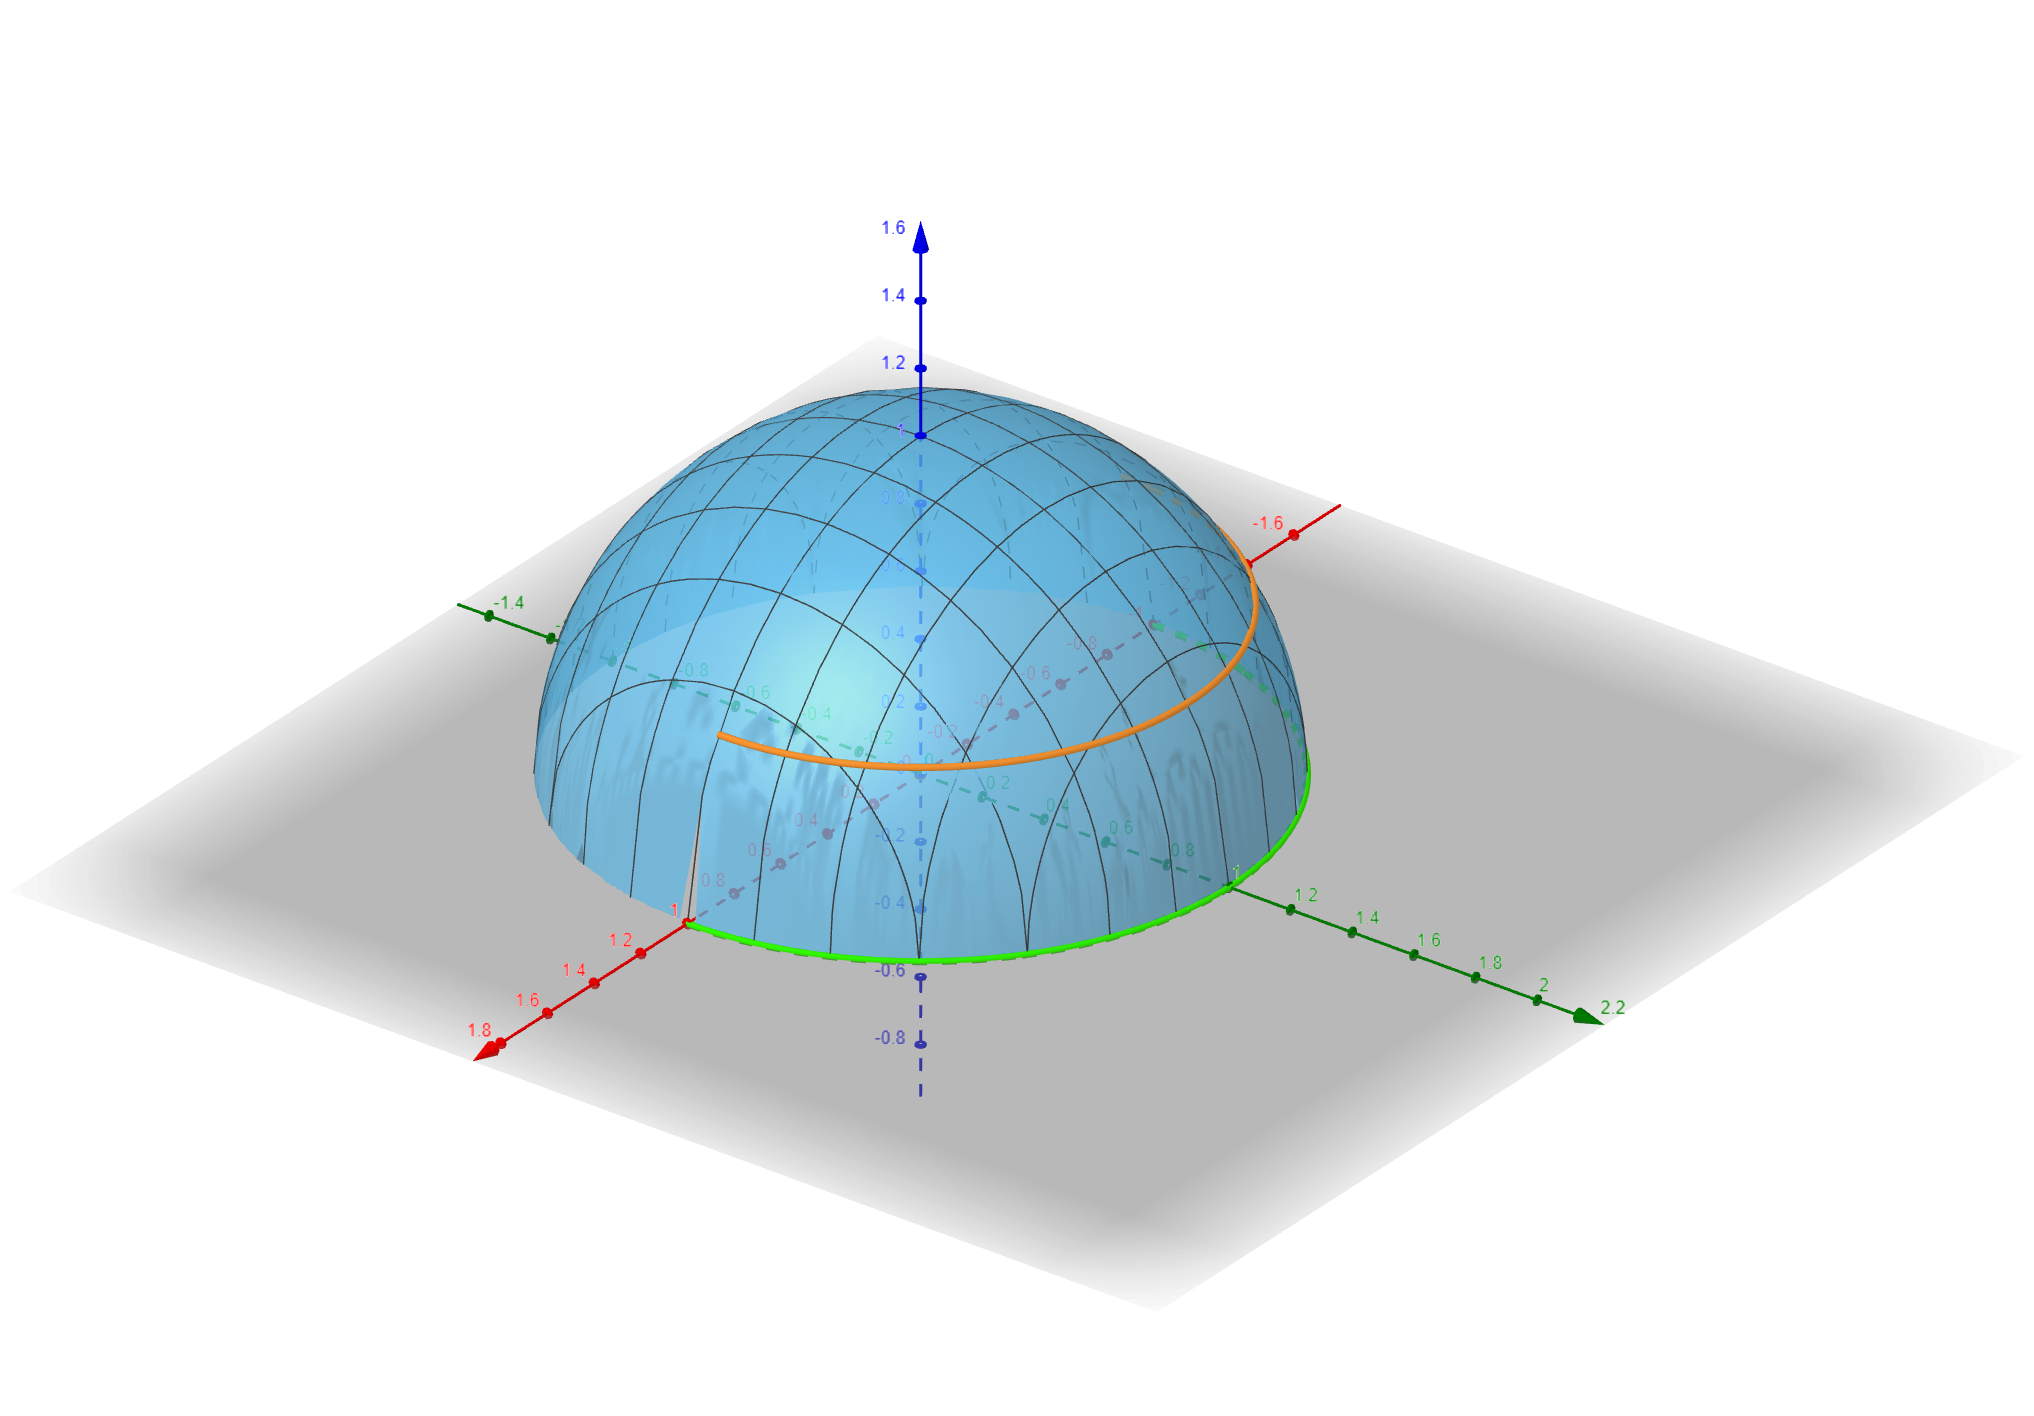
\includegraphics[scale=0.1]{Images/10.4.2.png}
				\centering
			\end{figure*}
		\end{enumerate}
		\newpage
		\item Sea $\set{x_k}\in \RR^n$ una sucesión cuyas coordenadas denotamos por
		\[x_k = \set{(x_k)_1,\cdots, (x_k)_n}.\]
		Prueba que
		\[x_k\rightarrow x = (x_1,\cdots,x_n) \quad \text{si y sólo si} \quad \pars{x_k}_i\rightarrow x_i, \quad \text{para toda $i:1,\cdots n$.}\]
		\begin{proof}
			Sea $\set{x_k}$ una sucesión tal que converge a $x$, entonces al ser $\Pi_i(x)$ la $i-esima$ proyección una función continua entonces
			
			\[\limtoinf{k} \pars{x_k}_i = \limtoinf{k} \Pi\pars{x_k} = \Pi\pars{\limtoinf{k} x_k} = \Pi\pars{x} = x_i,\]

			por lo que $\pars{x_k}_i$ converge a $x_i$ para toda $i:1,\cdots,n$.

			Ahora sean $\set{x_k}$ una sucesión tal que $\limtoinf{k} \pars{x_k}_i \rightarrow x_i$, luego por definición tenemos que para todo $\varepsilon>0$ existe un $N_i\in\NN$ tal que para todo $k\geq N$ se cumple que $\abs{\pars{x_k}_i - x_i}<\varepsilon$. Sea $N = \max\pars{N_1,\cdots,N_n}$ entonces

			\[\abs{\pars{x_k}_1 - x_1} + \cdots + \abs{\pars{x_k}_n - x_n} \leq \varepsilon,\]

			y por ser subaditividad y homogeneidad absoluta de la norma obtenemos

			\[\norm{x_k - x} = \norm{\sum_{i=1}^{N}\pars{\pars{x_k}_i - x_i}e_i} \leq \sum_{i=1}^{N}\norm{\pars{\pars{x_k}_i - x_i}e_i} = \sum_{i=1}^{N}\abs{\pars{x_k}_i - x_i}\norm{e_i} = \sum_{i=1}^{N}\abs{\pars{x_k}_i - x_i} < \varepsilon,\]

			donde $\set{e_1,\cdots, e_n}$ es la base canóninca de $\RR^n$. Por lo tanto $x_k$ converge a $x$.

			Con lo que concluimos que

			\[x_k\rightarrow x = (x_1,\cdots,x_n) \quad \text{si y sólo si} \quad \pars{x_k}_i\rightarrow x_i, \quad \text{para toda $i:1,\cdots n$.}\]

		\end{proof}
	\end{enumerate}
\end{document}

